% Options for packages loaded elsewhere
% Options for packages loaded elsewhere
\PassOptionsToPackage{unicode}{hyperref}
\PassOptionsToPackage{hyphens}{url}
\PassOptionsToPackage{dvipsnames,svgnames,x11names}{xcolor}
%
\documentclass[
  letterpaper,
  DIV=11,
  numbers=noendperiod]{scrartcl}
\usepackage{xcolor}
\usepackage{amsmath,amssymb}
\setcounter{secnumdepth}{-\maxdimen} % remove section numbering
\usepackage{iftex}
\ifPDFTeX
  \usepackage[T1]{fontenc}
  \usepackage[utf8]{inputenc}
  \usepackage{textcomp} % provide euro and other symbols
\else % if luatex or xetex
  \usepackage{unicode-math} % this also loads fontspec
  \defaultfontfeatures{Scale=MatchLowercase}
  \defaultfontfeatures[\rmfamily]{Ligatures=TeX,Scale=1}
\fi
\usepackage{lmodern}
\ifPDFTeX\else
  % xetex/luatex font selection
\fi
% Use upquote if available, for straight quotes in verbatim environments
\IfFileExists{upquote.sty}{\usepackage{upquote}}{}
\IfFileExists{microtype.sty}{% use microtype if available
  \usepackage[]{microtype}
  \UseMicrotypeSet[protrusion]{basicmath} % disable protrusion for tt fonts
}{}
\makeatletter
\@ifundefined{KOMAClassName}{% if non-KOMA class
  \IfFileExists{parskip.sty}{%
    \usepackage{parskip}
  }{% else
    \setlength{\parindent}{0pt}
    \setlength{\parskip}{6pt plus 2pt minus 1pt}}
}{% if KOMA class
  \KOMAoptions{parskip=half}}
\makeatother
% Make \paragraph and \subparagraph free-standing
\makeatletter
\ifx\paragraph\undefined\else
  \let\oldparagraph\paragraph
  \renewcommand{\paragraph}{
    \@ifstar
      \xxxParagraphStar
      \xxxParagraphNoStar
  }
  \newcommand{\xxxParagraphStar}[1]{\oldparagraph*{#1}\mbox{}}
  \newcommand{\xxxParagraphNoStar}[1]{\oldparagraph{#1}\mbox{}}
\fi
\ifx\subparagraph\undefined\else
  \let\oldsubparagraph\subparagraph
  \renewcommand{\subparagraph}{
    \@ifstar
      \xxxSubParagraphStar
      \xxxSubParagraphNoStar
  }
  \newcommand{\xxxSubParagraphStar}[1]{\oldsubparagraph*{#1}\mbox{}}
  \newcommand{\xxxSubParagraphNoStar}[1]{\oldsubparagraph{#1}\mbox{}}
\fi
\makeatother

\usepackage{color}
\usepackage{fancyvrb}
\newcommand{\VerbBar}{|}
\newcommand{\VERB}{\Verb[commandchars=\\\{\}]}
\DefineVerbatimEnvironment{Highlighting}{Verbatim}{commandchars=\\\{\}}
% Add ',fontsize=\small' for more characters per line
\usepackage{framed}
\definecolor{shadecolor}{RGB}{241,243,245}
\newenvironment{Shaded}{\begin{snugshade}}{\end{snugshade}}
\newcommand{\AlertTok}[1]{\textcolor[rgb]{0.68,0.00,0.00}{#1}}
\newcommand{\AnnotationTok}[1]{\textcolor[rgb]{0.37,0.37,0.37}{#1}}
\newcommand{\AttributeTok}[1]{\textcolor[rgb]{0.40,0.45,0.13}{#1}}
\newcommand{\BaseNTok}[1]{\textcolor[rgb]{0.68,0.00,0.00}{#1}}
\newcommand{\BuiltInTok}[1]{\textcolor[rgb]{0.00,0.23,0.31}{#1}}
\newcommand{\CharTok}[1]{\textcolor[rgb]{0.13,0.47,0.30}{#1}}
\newcommand{\CommentTok}[1]{\textcolor[rgb]{0.37,0.37,0.37}{#1}}
\newcommand{\CommentVarTok}[1]{\textcolor[rgb]{0.37,0.37,0.37}{\textit{#1}}}
\newcommand{\ConstantTok}[1]{\textcolor[rgb]{0.56,0.35,0.01}{#1}}
\newcommand{\ControlFlowTok}[1]{\textcolor[rgb]{0.00,0.23,0.31}{\textbf{#1}}}
\newcommand{\DataTypeTok}[1]{\textcolor[rgb]{0.68,0.00,0.00}{#1}}
\newcommand{\DecValTok}[1]{\textcolor[rgb]{0.68,0.00,0.00}{#1}}
\newcommand{\DocumentationTok}[1]{\textcolor[rgb]{0.37,0.37,0.37}{\textit{#1}}}
\newcommand{\ErrorTok}[1]{\textcolor[rgb]{0.68,0.00,0.00}{#1}}
\newcommand{\ExtensionTok}[1]{\textcolor[rgb]{0.00,0.23,0.31}{#1}}
\newcommand{\FloatTok}[1]{\textcolor[rgb]{0.68,0.00,0.00}{#1}}
\newcommand{\FunctionTok}[1]{\textcolor[rgb]{0.28,0.35,0.67}{#1}}
\newcommand{\ImportTok}[1]{\textcolor[rgb]{0.00,0.46,0.62}{#1}}
\newcommand{\InformationTok}[1]{\textcolor[rgb]{0.37,0.37,0.37}{#1}}
\newcommand{\KeywordTok}[1]{\textcolor[rgb]{0.00,0.23,0.31}{\textbf{#1}}}
\newcommand{\NormalTok}[1]{\textcolor[rgb]{0.00,0.23,0.31}{#1}}
\newcommand{\OperatorTok}[1]{\textcolor[rgb]{0.37,0.37,0.37}{#1}}
\newcommand{\OtherTok}[1]{\textcolor[rgb]{0.00,0.23,0.31}{#1}}
\newcommand{\PreprocessorTok}[1]{\textcolor[rgb]{0.68,0.00,0.00}{#1}}
\newcommand{\RegionMarkerTok}[1]{\textcolor[rgb]{0.00,0.23,0.31}{#1}}
\newcommand{\SpecialCharTok}[1]{\textcolor[rgb]{0.37,0.37,0.37}{#1}}
\newcommand{\SpecialStringTok}[1]{\textcolor[rgb]{0.13,0.47,0.30}{#1}}
\newcommand{\StringTok}[1]{\textcolor[rgb]{0.13,0.47,0.30}{#1}}
\newcommand{\VariableTok}[1]{\textcolor[rgb]{0.07,0.07,0.07}{#1}}
\newcommand{\VerbatimStringTok}[1]{\textcolor[rgb]{0.13,0.47,0.30}{#1}}
\newcommand{\WarningTok}[1]{\textcolor[rgb]{0.37,0.37,0.37}{\textit{#1}}}

\usepackage{longtable,booktabs,array}
\newcounter{none} % for unnumbered tables
\usepackage{calc} % for calculating minipage widths
% Correct order of tables after \paragraph or \subparagraph
\usepackage{etoolbox}
\makeatletter
\patchcmd\longtable{\par}{\if@noskipsec\mbox{}\fi\par}{}{}
\makeatother
% Allow footnotes in longtable head/foot
\IfFileExists{footnotehyper.sty}{\usepackage{footnotehyper}}{\usepackage{footnote}}
\makesavenoteenv{longtable}
\usepackage{graphicx}
\makeatletter
\newsavebox\pandoc@box
\newcommand*\pandocbounded[1]{% scales image to fit in text height/width
  \sbox\pandoc@box{#1}%
  \Gscale@div\@tempa{\textheight}{\dimexpr\ht\pandoc@box+\dp\pandoc@box\relax}%
  \Gscale@div\@tempb{\linewidth}{\wd\pandoc@box}%
  \ifdim\@tempb\p@<\@tempa\p@\let\@tempa\@tempb\fi% select the smaller of both
  \ifdim\@tempa\p@<\p@\scalebox{\@tempa}{\usebox\pandoc@box}%
  \else\usebox{\pandoc@box}%
  \fi%
}
% Set default figure placement to htbp
\def\fps@figure{htbp}
\makeatother





\setlength{\emergencystretch}{3em} % prevent overfull lines

\providecommand{\tightlist}{%
  \setlength{\itemsep}{0pt}\setlength{\parskip}{0pt}}



 


\KOMAoption{captions}{tableheading}
\makeatletter
\@ifpackageloaded{caption}{}{\usepackage{caption}}
\AtBeginDocument{%
\ifdefined\contentsname
  \renewcommand*\contentsname{Table of contents}
\else
  \newcommand\contentsname{Table of contents}
\fi
\ifdefined\listfigurename
  \renewcommand*\listfigurename{List of Figures}
\else
  \newcommand\listfigurename{List of Figures}
\fi
\ifdefined\listtablename
  \renewcommand*\listtablename{List of Tables}
\else
  \newcommand\listtablename{List of Tables}
\fi
\ifdefined\figurename
  \renewcommand*\figurename{Figure}
\else
  \newcommand\figurename{Figure}
\fi
\ifdefined\tablename
  \renewcommand*\tablename{Table}
\else
  \newcommand\tablename{Table}
\fi
}
\@ifpackageloaded{float}{}{\usepackage{float}}
\floatstyle{ruled}
\@ifundefined{c@chapter}{\newfloat{codelisting}{h}{lop}}{\newfloat{codelisting}{h}{lop}[chapter]}
\floatname{codelisting}{Listing}
\newcommand*\listoflistings{\listof{codelisting}{List of Listings}}
\makeatother
\makeatletter
\makeatother
\makeatletter
\@ifpackageloaded{caption}{}{\usepackage{caption}}
\@ifpackageloaded{subcaption}{}{\usepackage{subcaption}}
\makeatother
\usepackage{bookmark}
\IfFileExists{xurl.sty}{\usepackage{xurl}}{} % add URL line breaks if available
\urlstyle{same}
% fallback for those not using the hyperref driver hyperxmp:
\makeatletter
\@ifundefined{xmpquote}{\newcommand{\xmpquote}[1]{#1}}{}
\makeatother
\hypersetup{
  pdftitle={CS2 Dataset Overview and Initial Analysis},
  colorlinks=true,
  linkcolor={blue},
  filecolor={Maroon},
  citecolor={Blue},
  urlcolor={Blue},
  pdfcreator={LaTeX via pandoc}}


\title{CS2 Dataset Overview and Initial Analysis}
\usepackage{etoolbox}
\makeatletter
\providecommand{\subtitle}[1]{% add subtitle to \maketitle
  \apptocmd{\@title}{\par {\large #1 \par}}{}{}
}
\makeatother
\subtitle{Sections 2, 2.1, 2.2, 2.3, 3 and 4}
\author{}
\date{}
\begin{document}
\maketitle


\subsection{Setup}\label{setup}

This report reads the three Parquet datasets, prints descriptive tables
directly into the rendered report, and saves figures as PDF files in
\texttt{../reports/figures}.

\begin{Shaded}
\begin{Highlighting}[]
\FunctionTok{library}\NormalTok{(tidyverse)}
\FunctionTok{library}\NormalTok{(arrow)}
\FunctionTok{library}\NormalTok{(knitr)}

\CommentTok{\# Paths are relative to the directory containing this QMD file.}
\NormalTok{rounds\_file }\OtherTok{\textless{}{-}} \StringTok{"../data/analysis/rounds.parquet"}
\NormalTok{states\_file }\OtherTok{\textless{}{-}} \StringTok{"../data/analysis/round\_states.parquet"}
\NormalTok{enriched\_file }\OtherTok{\textless{}{-}} \StringTok{"../data/analysis/round\_states\_enriched.parquet"}

\NormalTok{figures\_dir }\OtherTok{\textless{}{-}} \StringTok{"../reports/figures"}
\FunctionTok{dir.create}\NormalTok{(figures\_dir, }\AttributeTok{showWarnings =} \ConstantTok{FALSE}\NormalTok{, }\AttributeTok{recursive =} \ConstantTok{TRUE}\NormalTok{)}

\NormalTok{rounds }\OtherTok{\textless{}{-}} \FunctionTok{read\_parquet}\NormalTok{(rounds\_file) }\SpecialCharTok{|\textgreater{}} \FunctionTok{as\_tibble}\NormalTok{()}
\NormalTok{round\_states }\OtherTok{\textless{}{-}} \FunctionTok{read\_parquet}\NormalTok{(states\_file) }\SpecialCharTok{|\textgreater{}} \FunctionTok{as\_tibble}\NormalTok{()}
\NormalTok{round\_states\_enriched }\OtherTok{\textless{}{-}} \FunctionTok{read\_parquet}\NormalTok{(enriched\_file) }\SpecialCharTok{|\textgreater{}} \FunctionTok{as\_tibble}\NormalTok{()}

\FunctionTok{stopifnot}\NormalTok{(}\FunctionTok{all}\NormalTok{(}\FunctionTok{c}\NormalTok{(}\StringTok{"match\_id"}\NormalTok{, }\StringTok{"map"}\NormalTok{, }\StringTok{"round\_num"}\NormalTok{) }\SpecialCharTok{\%in\%} \FunctionTok{names}\NormalTok{(rounds)))}
\FunctionTok{stopifnot}\NormalTok{(}\FunctionTok{all}\NormalTok{(}\FunctionTok{c}\NormalTok{(}\StringTok{"match\_id"}\NormalTok{, }\StringTok{"map"}\NormalTok{, }\StringTok{"round\_num"}\NormalTok{, }\StringTok{"tick"}\NormalTok{, }\StringTok{"seconds"}\NormalTok{,}
                \StringTok{"ct\_alive"}\NormalTok{, }\StringTok{"t\_alive"}\NormalTok{, }\StringTok{"ct\_win"}\NormalTok{) }\SpecialCharTok{\%in\%} \FunctionTok{names}\NormalTok{(round\_states)))}
\FunctionTok{stopifnot}\NormalTok{(}\FunctionTok{all}\NormalTok{(}\FunctionTok{c}\NormalTok{(}\StringTok{"match\_id"}\NormalTok{, }\StringTok{"map"}\NormalTok{, }\StringTok{"round\_num"}\NormalTok{) }\SpecialCharTok{\%in\%}
                \FunctionTok{names}\NormalTok{(round\_states\_enriched)))}

\CommentTok{\# Save each ggplot as a PDF.}
\NormalTok{save\_pdf }\OtherTok{\textless{}{-}} \ControlFlowTok{function}\NormalTok{(plot, filename, }\AttributeTok{width =} \DecValTok{9}\NormalTok{, }\AttributeTok{height =} \DecValTok{6}\NormalTok{) \{}
  \FunctionTok{ggsave}\NormalTok{(}
    \AttributeTok{filename =} \FunctionTok{file.path}\NormalTok{(figures\_dir, filename),}
    \AttributeTok{plot =}\NormalTok{ plot,}
    \AttributeTok{width =}\NormalTok{ width,}
    \AttributeTok{height =}\NormalTok{ height,}
    \AttributeTok{device =}\NormalTok{ grDevices}\SpecialCharTok{::}\NormalTok{cairo\_pdf}
\NormalTok{  )}
\NormalTok{\}}

\CommentTok{\# Consistent table display in the rendered report.}
\NormalTok{show\_table }\OtherTok{\textless{}{-}} \ControlFlowTok{function}\NormalTok{(x, }\AttributeTok{digits =} \DecValTok{2}\NormalTok{) \{}
\NormalTok{  knitr}\SpecialCharTok{::}\FunctionTok{kable}\NormalTok{(x, }\AttributeTok{digits =}\NormalTok{ digits, }\AttributeTok{format =} \StringTok{"html"}\NormalTok{)}
\NormalTok{\}}
\end{Highlighting}
\end{Shaded}

\subsection{2. Dataset structure}\label{dataset-structure}

\subsubsection{2.1 Overview of the three
datasets}\label{overview-of-the-three-datasets}

\begin{Shaded}
\begin{Highlighting}[]
\NormalTok{dataset\_overview }\OtherTok{\textless{}{-}} \FunctionTok{tibble}\NormalTok{(}
  \AttributeTok{dataset =} \FunctionTok{c}\NormalTok{(}\StringTok{"rounds"}\NormalTok{, }\StringTok{"round\_states"}\NormalTok{, }\StringTok{"round\_states\_enriched"}\NormalTok{),}
  \AttributeTok{rows =} \FunctionTok{c}\NormalTok{(}\FunctionTok{nrow}\NormalTok{(rounds), }\FunctionTok{nrow}\NormalTok{(round\_states), }\FunctionTok{nrow}\NormalTok{(round\_states\_enriched)),}
  \AttributeTok{columns =} \FunctionTok{c}\NormalTok{(}\FunctionTok{ncol}\NormalTok{(rounds), }\FunctionTok{ncol}\NormalTok{(round\_states), }\FunctionTok{ncol}\NormalTok{(round\_states\_enriched)),}
  \AttributeTok{missing\_cells =} \FunctionTok{c}\NormalTok{(}\FunctionTok{sum}\NormalTok{(}\FunctionTok{is.na}\NormalTok{(rounds)), }\FunctionTok{sum}\NormalTok{(}\FunctionTok{is.na}\NormalTok{(round\_states)),}
                    \FunctionTok{sum}\NormalTok{(}\FunctionTok{is.na}\NormalTok{(round\_states\_enriched))),}
  \AttributeTok{unique\_matches =} \FunctionTok{c}\NormalTok{(}\FunctionTok{n\_distinct}\NormalTok{(rounds}\SpecialCharTok{$}\NormalTok{match\_id),}
                     \FunctionTok{n\_distinct}\NormalTok{(round\_states}\SpecialCharTok{$}\NormalTok{match\_id),}
                     \FunctionTok{n\_distinct}\NormalTok{(round\_states\_enriched}\SpecialCharTok{$}\NormalTok{match\_id)),}
  \AttributeTok{unique\_rounds =} \FunctionTok{c}\NormalTok{(}
    \FunctionTok{nrow}\NormalTok{(}\FunctionTok{distinct}\NormalTok{(rounds, match\_id, round\_num)),}
    \FunctionTok{nrow}\NormalTok{(}\FunctionTok{distinct}\NormalTok{(round\_states, match\_id, round\_num)),}
    \FunctionTok{nrow}\NormalTok{(}\FunctionTok{distinct}\NormalTok{(round\_states\_enriched, match\_id, round\_num))}
\NormalTok{  )}
\NormalTok{)}
\FunctionTok{show\_table}\NormalTok{(dataset\_overview)}
\end{Highlighting}
\end{Shaded}

{\def\LTcaptype{none} % do not increment counter
\begin{longtable}[]{@{}lrrrrr@{}}
\toprule\noalign{}
dataset & rows & columns & missing\_cells & unique\_matches &
unique\_rounds \\
\midrule\noalign{}
\endhead
\bottomrule\noalign{}
\endlastfoot
rounds & 1257 & 26 & 1288 & 60 & 1257 \\
round\_states & 116201 & 45 & 195710 & 60 & 1257 \\
round\_states\_enriched & 116201 & 59 & 250917 & 60 & 1257 \\
\end{longtable}
}

\subsubsection{2.2 Column names and data
types}\label{column-names-and-data-types}

\begin{Shaded}
\begin{Highlighting}[]
\NormalTok{column\_overview }\OtherTok{\textless{}{-}} \FunctionTok{bind\_rows}\NormalTok{(}
  \FunctionTok{tibble}\NormalTok{(}\AttributeTok{dataset =} \StringTok{"rounds"}\NormalTok{, }\AttributeTok{column =} \FunctionTok{names}\NormalTok{(rounds),}
         \AttributeTok{data\_type =} \FunctionTok{map\_chr}\NormalTok{(rounds, }\SpecialCharTok{\textasciitilde{}} \FunctionTok{paste}\NormalTok{(}\FunctionTok{class}\NormalTok{(.x), }\AttributeTok{collapse =} \StringTok{"/"}\NormalTok{))),}
  \FunctionTok{tibble}\NormalTok{(}\AttributeTok{dataset =} \StringTok{"round\_states"}\NormalTok{, }\AttributeTok{column =} \FunctionTok{names}\NormalTok{(round\_states),}
         \AttributeTok{data\_type =} \FunctionTok{map\_chr}\NormalTok{(round\_states, }\SpecialCharTok{\textasciitilde{}} \FunctionTok{paste}\NormalTok{(}\FunctionTok{class}\NormalTok{(.x), }\AttributeTok{collapse =} \StringTok{"/"}\NormalTok{))),}
  \FunctionTok{tibble}\NormalTok{(}\AttributeTok{dataset =} \StringTok{"round\_states\_enriched"}\NormalTok{, }\AttributeTok{column =} \FunctionTok{names}\NormalTok{(round\_states\_enriched),}
         \AttributeTok{data\_type =} \FunctionTok{map\_chr}\NormalTok{(round\_states\_enriched,}
                             \SpecialCharTok{\textasciitilde{}} \FunctionTok{paste}\NormalTok{(}\FunctionTok{class}\NormalTok{(.x), }\AttributeTok{collapse =} \StringTok{"/"}\NormalTok{)))}
\NormalTok{)}
\FunctionTok{show\_table}\NormalTok{(column\_overview)}
\end{Highlighting}
\end{Shaded}

{\def\LTcaptype{none} % do not increment counter
\begin{longtable}[]{@{}lll@{}}
\toprule\noalign{}
dataset & column & data\_type \\
\midrule\noalign{}
\endhead
\bottomrule\noalign{}
\endlastfoot
rounds & match\_id & character \\
rounds & map & character \\
rounds & part & integer \\
rounds & round\_num & integer \\
rounds & is\_overtime & logical \\
rounds & is\_pistol\_round & logical \\
rounds & ct\_team & character \\
rounds & t\_team & character \\
rounds & ct\_score\_before & integer \\
rounds & t\_score\_before & integer \\
rounds & ct\_won\_previous\_round & logical \\
rounds & ct\_buy\_type & character \\
rounds & t\_buy\_type & character \\
rounds & ct\_equipment\_freeze\_end & integer \\
rounds & t\_equipment\_freeze\_end & integer \\
rounds & bomb\_planted & logical \\
rounds & plant\_site & character \\
rounds & first\_death\_side & character \\
rounds & freeze\_end\_tick & integer \\
rounds & plant\_tick & integer \\
rounds & end\_tick & integer \\
rounds & round\_duration\_s & numeric \\
rounds & winner\_side & character \\
rounds & winner\_team & character \\
rounds & ct\_win & logical \\
rounds & reason\_name & character \\
round\_states & match\_id & character \\
round\_states & map & character \\
round\_states & part & integer \\
round\_states & round\_num & integer \\
round\_states & tick & integer \\
round\_states & seconds & numeric \\
round\_states & time\_remaining\_s & numeric \\
round\_states & bomb\_planted & logical \\
round\_states & seconds\_since\_plant & numeric \\
round\_states & plant\_site & character \\
round\_states & bomb\_carried & logical \\
round\_states & ct\_team & character \\
round\_states & t\_team & character \\
round\_states & ct\_score\_before & integer \\
round\_states & t\_score\_before & integer \\
round\_states & ct\_alive & integer \\
round\_states & ct\_hp & integer \\
round\_states & ct\_armor & integer \\
round\_states & ct\_helmets & integer \\
round\_states & ct\_defusers & integer \\
round\_states & ct\_equipment & integer \\
round\_states & ct\_money & integer \\
round\_states & ct\_rifles & integer \\
round\_states & ct\_awps & integer \\
round\_states & ct\_smgs & integer \\
round\_states & ct\_smokes & integer \\
round\_states & ct\_flashes & integer \\
round\_states & ct\_he & integer \\
round\_states & ct\_molotovs & integer \\
round\_states & t\_alive & integer \\
round\_states & t\_hp & integer \\
round\_states & t\_armor & integer \\
round\_states & t\_helmets & integer \\
round\_states & t\_defusers & integer \\
round\_states & t\_equipment & integer \\
round\_states & t\_money & integer \\
round\_states & t\_rifles & integer \\
round\_states & t\_awps & integer \\
round\_states & t\_smgs & integer \\
round\_states & t\_smokes & integer \\
round\_states & t\_flashes & integer \\
round\_states & t\_he & integer \\
round\_states & t\_molotovs & integer \\
round\_states & winner\_side & character \\
round\_states & ct\_win & logical \\
round\_states\_enriched & match\_id & character \\
round\_states\_enriched & map & character \\
round\_states\_enriched & part & numeric \\
round\_states\_enriched & round\_num & numeric \\
round\_states\_enriched & tick & numeric \\
round\_states\_enriched & seconds & numeric \\
round\_states\_enriched & time\_remaining\_s & numeric \\
round\_states\_enriched & bomb\_planted & logical \\
round\_states\_enriched & seconds\_since\_plant & numeric \\
round\_states\_enriched & plant\_site & character \\
round\_states\_enriched & bomb\_carried & logical \\
round\_states\_enriched & ct\_team & character \\
round\_states\_enriched & t\_team & character \\
round\_states\_enriched & ct\_score\_before & numeric \\
round\_states\_enriched & t\_score\_before & numeric \\
round\_states\_enriched & ct\_alive & numeric \\
round\_states\_enriched & ct\_hp & numeric \\
round\_states\_enriched & ct\_armor & numeric \\
round\_states\_enriched & ct\_helmets & numeric \\
round\_states\_enriched & ct\_defusers & numeric \\
round\_states\_enriched & ct\_equipment & numeric \\
round\_states\_enriched & ct\_money & numeric \\
round\_states\_enriched & ct\_rifles & numeric \\
round\_states\_enriched & ct\_awps & numeric \\
round\_states\_enriched & ct\_smgs & numeric \\
round\_states\_enriched & ct\_smokes & numeric \\
round\_states\_enriched & ct\_flashes & numeric \\
round\_states\_enriched & ct\_he & numeric \\
round\_states\_enriched & ct\_molotovs & numeric \\
round\_states\_enriched & t\_alive & numeric \\
round\_states\_enriched & t\_hp & numeric \\
round\_states\_enriched & t\_armor & numeric \\
round\_states\_enriched & t\_helmets & numeric \\
round\_states\_enriched & t\_defusers & numeric \\
round\_states\_enriched & t\_equipment & numeric \\
round\_states\_enriched & t\_money & numeric \\
round\_states\_enriched & t\_rifles & numeric \\
round\_states\_enriched & t\_awps & numeric \\
round\_states\_enriched & t\_smgs & numeric \\
round\_states\_enriched & t\_smokes & numeric \\
round\_states\_enriched & t\_flashes & numeric \\
round\_states\_enriched & t\_he & numeric \\
round\_states\_enriched & t\_molotovs & numeric \\
round\_states\_enriched & winner\_side & character \\
round\_states\_enriched & ct\_win & logical \\
round\_states\_enriched & is\_overtime & logical \\
round\_states\_enriched & is\_pistol\_round & logical \\
round\_states\_enriched & ct\_won\_previous\_round & logical \\
round\_states\_enriched & ct\_buy\_type & character \\
round\_states\_enriched & t\_buy\_type & character \\
round\_states\_enriched & ct\_equipment\_freeze\_end & numeric \\
round\_states\_enriched & t\_equipment\_freeze\_end & numeric \\
round\_states\_enriched & first\_death\_side & character \\
round\_states\_enriched & freeze\_end\_tick & numeric \\
round\_states\_enriched & plant\_tick & numeric \\
round\_states\_enriched & end\_tick & numeric \\
round\_states\_enriched & round\_duration\_s & numeric \\
round\_states\_enriched & winner\_team & character \\
round\_states\_enriched & reason\_name & character \\
\end{longtable}
}

\subsubsection{2.3 Maps and teams}\label{maps-and-teams}

\begin{Shaded}
\begin{Highlighting}[]
\NormalTok{map\_overview }\OtherTok{\textless{}{-}}\NormalTok{ rounds }\SpecialCharTok{|\textgreater{}}
  \FunctionTok{group\_by}\NormalTok{(map) }\SpecialCharTok{|\textgreater{}}
  \FunctionTok{summarise}\NormalTok{(}\AttributeTok{rounds =} \FunctionTok{n}\NormalTok{(), }\AttributeTok{matches =} \FunctionTok{n\_distinct}\NormalTok{(match\_id), }\AttributeTok{.groups =} \StringTok{"drop"}\NormalTok{)}
\FunctionTok{show\_table}\NormalTok{(map\_overview)}
\end{Highlighting}
\end{Shaded}

{\def\LTcaptype{none} % do not increment counter
\begin{longtable}[]{@{}lrr@{}}
\toprule\noalign{}
map & rounds & matches \\
\midrule\noalign{}
\endhead
\bottomrule\noalign{}
\endlastfoot
de\_dust2 & 628 & 30 \\
de\_mirage & 629 & 30 \\
\end{longtable}
}

\begin{Shaded}
\begin{Highlighting}[]
\NormalTok{team\_overview }\OtherTok{\textless{}{-}} \FunctionTok{bind\_rows}\NormalTok{(}
\NormalTok{  rounds }\SpecialCharTok{|\textgreater{}} \FunctionTok{transmute}\NormalTok{(}\AttributeTok{team =}\NormalTok{ ct\_team),}
\NormalTok{  rounds }\SpecialCharTok{|\textgreater{}} \FunctionTok{transmute}\NormalTok{(}\AttributeTok{team =}\NormalTok{ t\_team)}
\NormalTok{) }\SpecialCharTok{|\textgreater{}}
  \FunctionTok{filter}\NormalTok{(}\SpecialCharTok{!}\FunctionTok{is.na}\NormalTok{(team)) }\SpecialCharTok{|\textgreater{}}
  \FunctionTok{distinct}\NormalTok{(team) }\SpecialCharTok{|\textgreater{}}
  \FunctionTok{arrange}\NormalTok{(team)}
\FunctionTok{show\_table}\NormalTok{(team\_overview)}
\end{Highlighting}
\end{Shaded}

{\def\LTcaptype{none} % do not increment counter
\begin{longtable}[]{@{}l@{}}
\toprule\noalign{}
team \\
\midrule\noalign{}
\endhead
\bottomrule\noalign{}
\endlastfoot
9z \\
Aurora \\
FURIA \\
FUT \\
FaZe \\
Falcons \\
G2 \\
Legacy \\
MOUZ \\
NAVI \\
Spirit \\
Vitality \\
\end{longtable}
}

\subsection{\texorpdfstring{2.1 Round-level data:
\texttt{rounds.parquet}}{2.1 Round-level data: rounds.parquet}}\label{round-level-data-rounds.parquet}

Each row is expected to represent one round.

\subsubsection{Duplicate round keys}\label{duplicate-round-keys}

\begin{Shaded}
\begin{Highlighting}[]
\NormalTok{round\_key\_check }\OtherTok{\textless{}{-}}\NormalTok{ rounds }\SpecialCharTok{|\textgreater{}}
  \FunctionTok{count}\NormalTok{(match\_id, round\_num, }\AttributeTok{name =} \StringTok{"rows\_per\_round"}\NormalTok{) }\SpecialCharTok{|\textgreater{}}
  \FunctionTok{filter}\NormalTok{(rows\_per\_round }\SpecialCharTok{\textgreater{}} \DecValTok{1}\NormalTok{)}

\FunctionTok{tibble}\NormalTok{(}\AttributeTok{duplicate\_round\_keys =} \FunctionTok{nrow}\NormalTok{(round\_key\_check)) }\SpecialCharTok{|\textgreater{}} \FunctionTok{show\_table}\NormalTok{()}
\end{Highlighting}
\end{Shaded}

{\def\LTcaptype{none} % do not increment counter
\begin{longtable}[]{@{}r@{}}
\toprule\noalign{}
duplicate\_round\_keys \\
\midrule\noalign{}
\endhead
\bottomrule\noalign{}
\endlastfoot
0 \\
\end{longtable}
}

\begin{Shaded}
\begin{Highlighting}[]
\ControlFlowTok{if}\NormalTok{ (}\FunctionTok{nrow}\NormalTok{(round\_key\_check) }\SpecialCharTok{\textgreater{}} \DecValTok{0}\NormalTok{) }\FunctionTok{show\_table}\NormalTok{(round\_key\_check)}
\end{Highlighting}
\end{Shaded}

\subsubsection{Round summary by map}\label{round-summary-by-map}

\begin{Shaded}
\begin{Highlighting}[]
\NormalTok{rounds\_by\_map }\OtherTok{\textless{}{-}}\NormalTok{ rounds }\SpecialCharTok{|\textgreater{}}
  \FunctionTok{group\_by}\NormalTok{(map) }\SpecialCharTok{|\textgreater{}}
  \FunctionTok{summarise}\NormalTok{(}
    \AttributeTok{rounds =} \FunctionTok{n}\NormalTok{(),}
    \AttributeTok{matches =} \FunctionTok{n\_distinct}\NormalTok{(match\_id),}
    \AttributeTok{pistol\_rounds =} \FunctionTok{sum}\NormalTok{(is\_pistol\_round }\SpecialCharTok{\%in\%} \ConstantTok{TRUE}\NormalTok{, }\AttributeTok{na.rm =} \ConstantTok{TRUE}\NormalTok{),}
    \AttributeTok{overtime\_rounds =} \FunctionTok{sum}\NormalTok{(is\_overtime }\SpecialCharTok{\%in\%} \ConstantTok{TRUE}\NormalTok{, }\AttributeTok{na.rm =} \ConstantTok{TRUE}\NormalTok{),}
    \AttributeTok{planted\_rounds =} \FunctionTok{sum}\NormalTok{(bomb\_planted }\SpecialCharTok{\%in\%} \ConstantTok{TRUE}\NormalTok{, }\AttributeTok{na.rm =} \ConstantTok{TRUE}\NormalTok{),}
    \AttributeTok{planted\_pct =} \DecValTok{100} \SpecialCharTok{*} \FunctionTok{mean}\NormalTok{(bomb\_planted }\SpecialCharTok{\%in\%} \ConstantTok{TRUE}\NormalTok{, }\AttributeTok{na.rm =} \ConstantTok{TRUE}\NormalTok{),}
    \AttributeTok{mean\_duration\_s =} \FunctionTok{mean}\NormalTok{(round\_duration\_s, }\AttributeTok{na.rm =} \ConstantTok{TRUE}\NormalTok{),}
    \AttributeTok{median\_duration\_s =} \FunctionTok{median}\NormalTok{(round\_duration\_s, }\AttributeTok{na.rm =} \ConstantTok{TRUE}\NormalTok{),}
    \AttributeTok{.groups =} \StringTok{"drop"}
\NormalTok{  )}
\FunctionTok{show\_table}\NormalTok{(rounds\_by\_map)}
\end{Highlighting}
\end{Shaded}

{\def\LTcaptype{none} % do not increment counter
\begin{longtable}[]{@{}lrrrrrrrr@{}}
\toprule\noalign{}
map & rounds & matches & pistol\_rounds & overtime\_rounds &
planted\_rounds & planted\_pct & mean\_duration\_s &
median\_duration\_s \\
\midrule\noalign{}
\endhead
\bottomrule\noalign{}
\endlastfoot
de\_dust2 & 628 & 30 & 60 & 14 & 349 & 55.57 & 94.20 & 96.73 \\
de\_mirage & 629 & 30 & 60 & 16 & 312 & 49.60 & 89.75 & 91.30 \\
\end{longtable}
}

\subsubsection{Match length}\label{match-length}

\begin{Shaded}
\begin{Highlighting}[]
\NormalTok{rounds\_per\_match }\OtherTok{\textless{}{-}}\NormalTok{ rounds }\SpecialCharTok{|\textgreater{}}
  \FunctionTok{distinct}\NormalTok{(match\_id, map, round\_num) }\SpecialCharTok{|\textgreater{}}
  \FunctionTok{count}\NormalTok{(match\_id, map, }\AttributeTok{name =} \StringTok{"rounds\_in\_match"}\NormalTok{)}

\NormalTok{match\_length\_summary }\OtherTok{\textless{}{-}}\NormalTok{ rounds\_per\_match }\SpecialCharTok{|\textgreater{}}
  \FunctionTok{summarise}\NormalTok{(}
    \AttributeTok{matches =} \FunctionTok{n}\NormalTok{(),}
    \AttributeTok{min\_rounds =} \FunctionTok{min}\NormalTok{(rounds\_in\_match),}
    \AttributeTok{q1\_rounds =} \FunctionTok{quantile}\NormalTok{(rounds\_in\_match, }\FloatTok{0.25}\NormalTok{),}
    \AttributeTok{median\_rounds =} \FunctionTok{median}\NormalTok{(rounds\_in\_match),}
    \AttributeTok{mean\_rounds =} \FunctionTok{mean}\NormalTok{(rounds\_in\_match),}
    \AttributeTok{q3\_rounds =} \FunctionTok{quantile}\NormalTok{(rounds\_in\_match, }\FloatTok{0.75}\NormalTok{),}
    \AttributeTok{max\_rounds =} \FunctionTok{max}\NormalTok{(rounds\_in\_match)}
\NormalTok{  )}
\FunctionTok{show\_table}\NormalTok{(match\_length\_summary)}
\end{Highlighting}
\end{Shaded}

{\def\LTcaptype{none} % do not increment counter
\begin{longtable}[]{@{}rrrrrrr@{}}
\toprule\noalign{}
matches & min\_rounds & q1\_rounds & median\_rounds & mean\_rounds &
q3\_rounds & max\_rounds \\
\midrule\noalign{}
\endhead
\bottomrule\noalign{}
\endlastfoot
60 & 14 & 18.75 & 21 & 20.95 & 22.25 & 35 \\
\end{longtable}
}

\subsubsection{Round outcomes by map and winning
side}\label{round-outcomes-by-map-and-winning-side}

\begin{Shaded}
\begin{Highlighting}[]
\NormalTok{round\_outcomes }\OtherTok{\textless{}{-}}\NormalTok{ rounds }\SpecialCharTok{|\textgreater{}}
  \FunctionTok{count}\NormalTok{(map, winner\_side, }\AttributeTok{name =} \StringTok{"rounds"}\NormalTok{) }\SpecialCharTok{|\textgreater{}}
  \FunctionTok{group\_by}\NormalTok{(map) }\SpecialCharTok{|\textgreater{}}
  \FunctionTok{mutate}\NormalTok{(}\AttributeTok{percentage =} \DecValTok{100} \SpecialCharTok{*}\NormalTok{ rounds }\SpecialCharTok{/} \FunctionTok{sum}\NormalTok{(rounds)) }\SpecialCharTok{|\textgreater{}}
  \FunctionTok{ungroup}\NormalTok{()}

\FunctionTok{show\_table}\NormalTok{(round\_outcomes)}
\end{Highlighting}
\end{Shaded}

{\def\LTcaptype{none} % do not increment counter
\begin{longtable}[]{@{}llrr@{}}
\toprule\noalign{}
map & winner\_side & rounds & percentage \\
\midrule\noalign{}
\endhead
\bottomrule\noalign{}
\endlastfoot
de\_dust2 & counter-terrorist & 312 & 49.68 \\
de\_dust2 & terrorist & 316 & 50.32 \\
de\_mirage & counter-terrorist & 351 & 55.80 \\
de\_mirage & terrorist & 278 & 44.20 \\
\end{longtable}
}

\begin{Shaded}
\begin{Highlighting}[]
\NormalTok{p\_round\_outcomes }\OtherTok{\textless{}{-}} \FunctionTok{ggplot}\NormalTok{(}
\NormalTok{  round\_outcomes, }\FunctionTok{aes}\NormalTok{(}\AttributeTok{x =}\NormalTok{ map, }\AttributeTok{y =}\NormalTok{ percentage, }\AttributeTok{fill =}\NormalTok{ winner\_side)}
\NormalTok{) }\SpecialCharTok{+}
  \FunctionTok{geom\_col}\NormalTok{() }\SpecialCharTok{+}
  \FunctionTok{geom\_text}\NormalTok{(}\FunctionTok{aes}\NormalTok{(}\AttributeTok{label =} \FunctionTok{sprintf}\NormalTok{(}\StringTok{"\%.1f\%\%"}\NormalTok{, percentage)),}
            \AttributeTok{position =} \FunctionTok{position\_stack}\NormalTok{(}\AttributeTok{vjust =} \FloatTok{0.5}\NormalTok{), }\AttributeTok{size =} \FloatTok{3.5}\NormalTok{) }\SpecialCharTok{+}
  \FunctionTok{labs}\NormalTok{(}\AttributeTok{title =} \StringTok{"Round outcomes by map"}\NormalTok{, }\AttributeTok{x =} \StringTok{"Map"}\NormalTok{,}
       \AttributeTok{y =} \StringTok{"Percentage of rounds"}\NormalTok{, }\AttributeTok{fill =} \StringTok{"Winning side"}\NormalTok{) }\SpecialCharTok{+}
  \FunctionTok{theme\_minimal}\NormalTok{()}

\NormalTok{p\_round\_outcomes}
\end{Highlighting}
\end{Shaded}

\pandocbounded{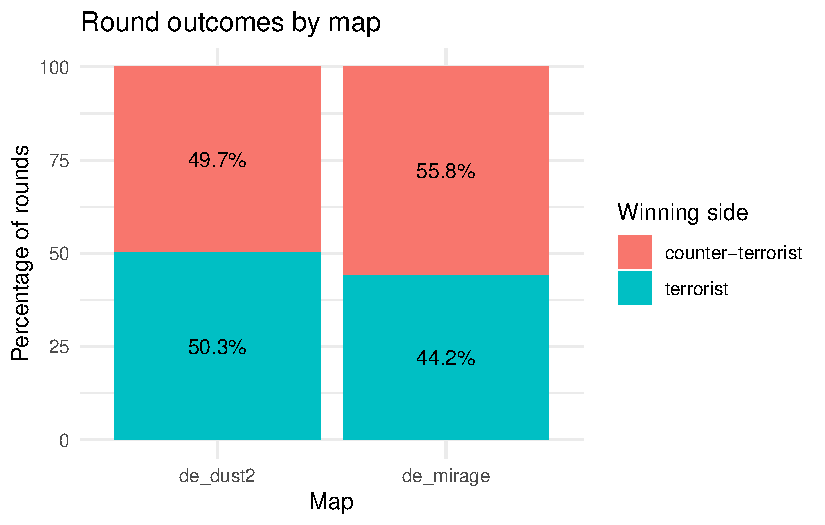
\includegraphics[keepaspectratio]{cs2_dataset_overview_files/figure-pdf/unnamed-chunk-8-1.pdf}}

\begin{Shaded}
\begin{Highlighting}[]
\FunctionTok{save\_pdf}\NormalTok{(p\_round\_outcomes, }\StringTok{"21\_round\_outcomes\_by\_map.pdf"}\NormalTok{)}
\end{Highlighting}
\end{Shaded}

\subsection{\texorpdfstring{2.2 Round-state data:
\texttt{round\_states.parquet}}{2.2 Round-state data: round\_states.parquet}}\label{round-state-data-round_states.parquet}

Each row is a snapshot of a round at a particular time. Snapshots from
the same round are repeated observations, not independent rounds.

\subsubsection{Snapshots per round}\label{snapshots-per-round}

\begin{Shaded}
\begin{Highlighting}[]
\NormalTok{snapshots\_per\_round }\OtherTok{\textless{}{-}}\NormalTok{ round\_states }\SpecialCharTok{|\textgreater{}}
  \FunctionTok{count}\NormalTok{(match\_id, map, round\_num, }\AttributeTok{name =} \StringTok{"snapshots"}\NormalTok{)}

\NormalTok{snapshot\_count\_summary }\OtherTok{\textless{}{-}}\NormalTok{ snapshots\_per\_round }\SpecialCharTok{|\textgreater{}}
  \FunctionTok{summarise}\NormalTok{(}
    \AttributeTok{rounds =} \FunctionTok{n}\NormalTok{(),}
    \AttributeTok{min\_snapshots =} \FunctionTok{min}\NormalTok{(snapshots),}
    \AttributeTok{q1\_snapshots =} \FunctionTok{quantile}\NormalTok{(snapshots, }\FloatTok{0.25}\NormalTok{),}
    \AttributeTok{median\_snapshots =} \FunctionTok{median}\NormalTok{(snapshots),}
    \AttributeTok{mean\_snapshots =} \FunctionTok{mean}\NormalTok{(snapshots),}
    \AttributeTok{q3\_snapshots =} \FunctionTok{quantile}\NormalTok{(snapshots, }\FloatTok{0.75}\NormalTok{),}
    \AttributeTok{max\_snapshots =} \FunctionTok{max}\NormalTok{(snapshots)}
\NormalTok{  )}
\FunctionTok{show\_table}\NormalTok{(snapshot\_count\_summary)}
\end{Highlighting}
\end{Shaded}

{\def\LTcaptype{none} % do not increment counter
\begin{longtable}[]{@{}rrrrrrr@{}}
\toprule\noalign{}
rounds & min\_snapshots & q1\_snapshots & median\_snapshots &
mean\_snapshots & q3\_snapshots & max\_snapshots \\
\midrule\noalign{}
\endhead
\bottomrule\noalign{}
\endlastfoot
1257 & 14 & 71 & 95 & 92.44 & 115 & 156 \\
\end{longtable}
}

\subsubsection{Snapshot timing and missing
values}\label{snapshot-timing-and-missing-values}

\begin{Shaded}
\begin{Highlighting}[]
\NormalTok{snapshot\_timing }\OtherTok{\textless{}{-}}\NormalTok{ round\_states }\SpecialCharTok{|\textgreater{}}
  \FunctionTok{summarise}\NormalTok{(}
    \AttributeTok{min\_seconds =} \FunctionTok{min}\NormalTok{(seconds, }\AttributeTok{na.rm =} \ConstantTok{TRUE}\NormalTok{),}
    \AttributeTok{median\_seconds =} \FunctionTok{median}\NormalTok{(seconds, }\AttributeTok{na.rm =} \ConstantTok{TRUE}\NormalTok{),}
    \AttributeTok{max\_seconds =} \FunctionTok{max}\NormalTok{(seconds, }\AttributeTok{na.rm =} \ConstantTok{TRUE}\NormalTok{),}
    \AttributeTok{min\_time\_remaining =} \FunctionTok{min}\NormalTok{(time\_remaining\_s, }\AttributeTok{na.rm =} \ConstantTok{TRUE}\NormalTok{),}
    \AttributeTok{max\_time\_remaining =} \FunctionTok{max}\NormalTok{(time\_remaining\_s, }\AttributeTok{na.rm =} \ConstantTok{TRUE}\NormalTok{)}
\NormalTok{  )}
\FunctionTok{show\_table}\NormalTok{(snapshot\_timing)}
\end{Highlighting}
\end{Shaded}

{\def\LTcaptype{none} % do not increment counter
\begin{longtable}[]{@{}rrrrr@{}}
\toprule\noalign{}
min\_seconds & median\_seconds & max\_seconds & min\_time\_remaining &
max\_time\_remaining \\
\midrule\noalign{}
\endhead
\bottomrule\noalign{}
\endlastfoot
0 & 46 & 155 & -0.98 & 115.2 \\
\end{longtable}
}

\begin{Shaded}
\begin{Highlighting}[]
\NormalTok{snapshot\_missingness }\OtherTok{\textless{}{-}} \FunctionTok{tibble}\NormalTok{(}
  \AttributeTok{column =} \FunctionTok{names}\NormalTok{(round\_states),}
  \AttributeTok{missing\_values =} \FunctionTok{map\_int}\NormalTok{(round\_states, }\SpecialCharTok{\textasciitilde{}} \FunctionTok{sum}\NormalTok{(}\FunctionTok{is.na}\NormalTok{(.x))),}
  \AttributeTok{missing\_pct =} \DecValTok{100} \SpecialCharTok{*}\NormalTok{ missing\_values }\SpecialCharTok{/} \FunctionTok{nrow}\NormalTok{(round\_states)}
\NormalTok{) }\SpecialCharTok{|\textgreater{}}
  \FunctionTok{arrange}\NormalTok{(}\FunctionTok{desc}\NormalTok{(missing\_values))}
\FunctionTok{show\_table}\NormalTok{(snapshot\_missingness)}
\end{Highlighting}
\end{Shaded}

{\def\LTcaptype{none} % do not increment counter
\begin{longtable}[]{@{}lrr@{}}
\toprule\noalign{}
column & missing\_values & missing\_pct \\
\midrule\noalign{}
\endhead
\bottomrule\noalign{}
\endlastfoot
seconds\_since\_plant & 97855 & 84.21 \\
plant\_site & 97855 & 84.21 \\
match\_id & 0 & 0.00 \\
map & 0 & 0.00 \\
part & 0 & 0.00 \\
round\_num & 0 & 0.00 \\
tick & 0 & 0.00 \\
seconds & 0 & 0.00 \\
time\_remaining\_s & 0 & 0.00 \\
bomb\_planted & 0 & 0.00 \\
bomb\_carried & 0 & 0.00 \\
ct\_team & 0 & 0.00 \\
t\_team & 0 & 0.00 \\
ct\_score\_before & 0 & 0.00 \\
t\_score\_before & 0 & 0.00 \\
ct\_alive & 0 & 0.00 \\
ct\_hp & 0 & 0.00 \\
ct\_armor & 0 & 0.00 \\
ct\_helmets & 0 & 0.00 \\
ct\_defusers & 0 & 0.00 \\
ct\_equipment & 0 & 0.00 \\
ct\_money & 0 & 0.00 \\
ct\_rifles & 0 & 0.00 \\
ct\_awps & 0 & 0.00 \\
ct\_smgs & 0 & 0.00 \\
ct\_smokes & 0 & 0.00 \\
ct\_flashes & 0 & 0.00 \\
ct\_he & 0 & 0.00 \\
ct\_molotovs & 0 & 0.00 \\
t\_alive & 0 & 0.00 \\
t\_hp & 0 & 0.00 \\
t\_armor & 0 & 0.00 \\
t\_helmets & 0 & 0.00 \\
t\_defusers & 0 & 0.00 \\
t\_equipment & 0 & 0.00 \\
t\_money & 0 & 0.00 \\
t\_rifles & 0 & 0.00 \\
t\_awps & 0 & 0.00 \\
t\_smgs & 0 & 0.00 \\
t\_smokes & 0 & 0.00 \\
t\_flashes & 0 & 0.00 \\
t\_he & 0 & 0.00 \\
t\_molotovs & 0 & 0.00 \\
winner\_side & 0 & 0.00 \\
ct\_win & 0 & 0.00 \\
\end{longtable}
}

\subsubsection{Alive-player advantage and eventual
outcome}\label{alive-player-advantage-and-eventual-outcome}

This is a snapshot-level exploratory comparison. Because the same round
contributes multiple snapshots, the percentages below should not be
interpreted as independent-round estimates.

\begin{Shaded}
\begin{Highlighting}[]
\NormalTok{state\_advantage }\OtherTok{\textless{}{-}}\NormalTok{ round\_states }\SpecialCharTok{|\textgreater{}}
  \FunctionTok{mutate}\NormalTok{(}
    \AttributeTok{alive\_difference =}\NormalTok{ ct\_alive }\SpecialCharTok{{-}}\NormalTok{ t\_alive,}
    \AttributeTok{alive\_advantage =} \FunctionTok{case\_when}\NormalTok{(}
\NormalTok{      alive\_difference }\SpecialCharTok{\textgreater{}} \DecValTok{0} \SpecialCharTok{\textasciitilde{}} \StringTok{"CT advantage"}\NormalTok{,}
\NormalTok{      alive\_difference }\SpecialCharTok{\textless{}} \DecValTok{0} \SpecialCharTok{\textasciitilde{}} \StringTok{"T advantage"}\NormalTok{,}
\NormalTok{      alive\_difference }\SpecialCharTok{==} \DecValTok{0} \SpecialCharTok{\textasciitilde{}} \StringTok{"Equal alive players"}\NormalTok{,}
      \ConstantTok{TRUE} \SpecialCharTok{\textasciitilde{}} \ConstantTok{NA\_character\_}
\NormalTok{    )}
\NormalTok{  )}

\NormalTok{advantage\_by\_outcome }\OtherTok{\textless{}{-}}\NormalTok{ state\_advantage }\SpecialCharTok{|\textgreater{}}
  \FunctionTok{filter}\NormalTok{(}\SpecialCharTok{!}\FunctionTok{is.na}\NormalTok{(ct\_win), }\SpecialCharTok{!}\FunctionTok{is.na}\NormalTok{(alive\_advantage)) }\SpecialCharTok{|\textgreater{}}
  \FunctionTok{group\_by}\NormalTok{(alive\_advantage) }\SpecialCharTok{|\textgreater{}}
  \FunctionTok{summarise}\NormalTok{(}
    \AttributeTok{snapshots =} \FunctionTok{n}\NormalTok{(),}
    \AttributeTok{ct\_round\_win\_pct =} \DecValTok{100} \SpecialCharTok{*} \FunctionTok{mean}\NormalTok{(ct\_win, }\AttributeTok{na.rm =} \ConstantTok{TRUE}\NormalTok{),}
    \AttributeTok{.groups =} \StringTok{"drop"}
\NormalTok{  )}
\FunctionTok{show\_table}\NormalTok{(advantage\_by\_outcome)}
\end{Highlighting}
\end{Shaded}

{\def\LTcaptype{none} % do not increment counter
\begin{longtable}[]{@{}lrr@{}}
\toprule\noalign{}
alive\_advantage & snapshots & ct\_round\_win\_pct \\
\midrule\noalign{}
\endhead
\bottomrule\noalign{}
\endlastfoot
CT advantage & 28565 & 83.42 \\
Equal alive players & 60682 & 50.68 \\
T advantage & 26954 & 10.40 \\
\end{longtable}
}

\begin{Shaded}
\begin{Highlighting}[]
\NormalTok{p\_alive\_advantage }\OtherTok{\textless{}{-}} \FunctionTok{ggplot}\NormalTok{(}
\NormalTok{  advantage\_by\_outcome, }\FunctionTok{aes}\NormalTok{(}\AttributeTok{x =}\NormalTok{ alive\_advantage, }\AttributeTok{y =}\NormalTok{ ct\_round\_win\_pct)}
\NormalTok{) }\SpecialCharTok{+}
  \FunctionTok{geom\_col}\NormalTok{() }\SpecialCharTok{+}
  \FunctionTok{geom\_text}\NormalTok{(}\FunctionTok{aes}\NormalTok{(}\AttributeTok{label =} \FunctionTok{sprintf}\NormalTok{(}\StringTok{"\%.1f\%\%"}\NormalTok{, ct\_round\_win\_pct)), }\AttributeTok{vjust =} \SpecialCharTok{{-}}\FloatTok{0.3}\NormalTok{) }\SpecialCharTok{+}
  \FunctionTok{scale\_y\_continuous}\NormalTok{(}\AttributeTok{limits =} \FunctionTok{c}\NormalTok{(}\DecValTok{0}\NormalTok{, }\DecValTok{100}\NormalTok{),}
                     \AttributeTok{expand =} \FunctionTok{expansion}\NormalTok{(}\AttributeTok{mult =} \FunctionTok{c}\NormalTok{(}\DecValTok{0}\NormalTok{, }\FloatTok{0.08}\NormalTok{))) }\SpecialCharTok{+}
  \FunctionTok{labs}\NormalTok{(}\AttributeTok{title =} \StringTok{"CT round{-}win percentage by alive{-}player advantage"}\NormalTok{,}
       \AttributeTok{subtitle =} \StringTok{"Snapshot{-}level descriptive comparison"}\NormalTok{,}
       \AttributeTok{x =} \StringTok{"Player{-}count state"}\NormalTok{, }\AttributeTok{y =} \StringTok{"CT round wins (\%)"}\NormalTok{) }\SpecialCharTok{+}
  \FunctionTok{theme\_minimal}\NormalTok{() }\SpecialCharTok{+}
  \FunctionTok{theme}\NormalTok{(}\AttributeTok{axis.text.x =} \FunctionTok{element\_text}\NormalTok{(}\AttributeTok{angle =} \DecValTok{15}\NormalTok{, }\AttributeTok{hjust =} \DecValTok{1}\NormalTok{))}

\NormalTok{p\_alive\_advantage}
\end{Highlighting}
\end{Shaded}

\pandocbounded{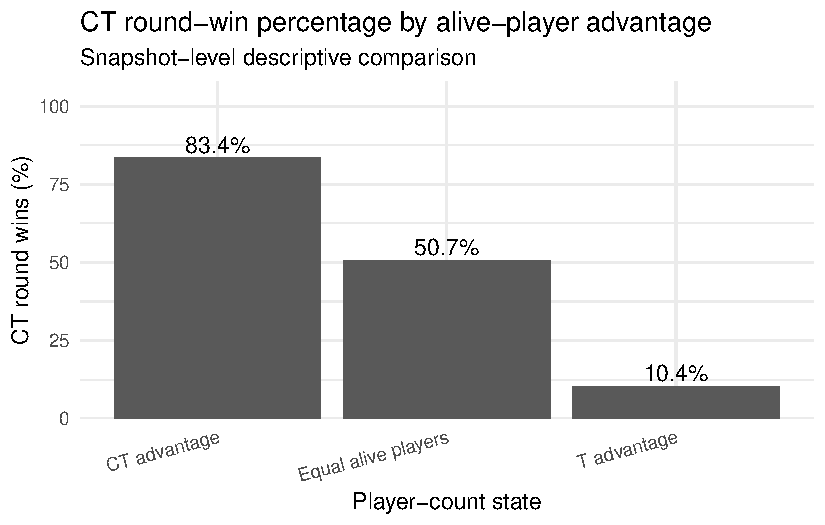
\includegraphics[keepaspectratio]{cs2_dataset_overview_files/figure-pdf/unnamed-chunk-11-1.pdf}}

\begin{Shaded}
\begin{Highlighting}[]
\FunctionTok{save\_pdf}\NormalTok{(p\_alive\_advantage, }\StringTok{"22\_alive\_advantage\_by\_outcome.pdf"}\NormalTok{)}
\end{Highlighting}
\end{Shaded}

\subsection{2.3 Enriched round-state
data}\label{enriched-round-state-data}

\subsubsection{Check row counts and round
keys}\label{check-row-counts-and-round-keys}

\begin{Shaded}
\begin{Highlighting}[]
\NormalTok{enrichment\_comparison }\OtherTok{\textless{}{-}} \FunctionTok{tibble}\NormalTok{(}
  \AttributeTok{dataset =} \FunctionTok{c}\NormalTok{(}\StringTok{"round\_states"}\NormalTok{, }\StringTok{"round\_states\_enriched"}\NormalTok{),}
  \AttributeTok{rows =} \FunctionTok{c}\NormalTok{(}\FunctionTok{nrow}\NormalTok{(round\_states), }\FunctionTok{nrow}\NormalTok{(round\_states\_enriched)),}
  \AttributeTok{columns =} \FunctionTok{c}\NormalTok{(}\FunctionTok{ncol}\NormalTok{(round\_states), }\FunctionTok{ncol}\NormalTok{(round\_states\_enriched)),}
  \AttributeTok{unique\_rounds =} \FunctionTok{c}\NormalTok{(}
    \FunctionTok{nrow}\NormalTok{(}\FunctionTok{distinct}\NormalTok{(round\_states, match\_id, round\_num)),}
    \FunctionTok{nrow}\NormalTok{(}\FunctionTok{distinct}\NormalTok{(round\_states\_enriched, match\_id, round\_num))}
\NormalTok{  )}
\NormalTok{)}
\FunctionTok{show\_table}\NormalTok{(enrichment\_comparison)}
\end{Highlighting}
\end{Shaded}

{\def\LTcaptype{none} % do not increment counter
\begin{longtable}[]{@{}lrrr@{}}
\toprule\noalign{}
dataset & rows & columns & unique\_rounds \\
\midrule\noalign{}
\endhead
\bottomrule\noalign{}
\endlastfoot
round\_states & 116201 & 45 & 1257 \\
round\_states\_enriched & 116201 & 59 & 1257 \\
\end{longtable}
}

\begin{Shaded}
\begin{Highlighting}[]
\NormalTok{snapshot\_key\_check }\OtherTok{\textless{}{-}}\NormalTok{ round\_states\_enriched }\SpecialCharTok{|\textgreater{}}
  \FunctionTok{count}\NormalTok{(match\_id, round\_num, tick, }\AttributeTok{name =} \StringTok{"rows\_per\_snapshot"}\NormalTok{) }\SpecialCharTok{|\textgreater{}}
  \FunctionTok{filter}\NormalTok{(rows\_per\_snapshot }\SpecialCharTok{\textgreater{}} \DecValTok{1}\NormalTok{)}

\FunctionTok{tibble}\NormalTok{(}\AttributeTok{duplicate\_match\_round\_tick\_keys =} \FunctionTok{nrow}\NormalTok{(snapshot\_key\_check)) }\SpecialCharTok{|\textgreater{}}
  \FunctionTok{show\_table}\NormalTok{()}
\end{Highlighting}
\end{Shaded}

{\def\LTcaptype{none} % do not increment counter
\begin{longtable}[]{@{}r@{}}
\toprule\noalign{}
duplicate\_match\_round\_tick\_keys \\
\midrule\noalign{}
\endhead
\bottomrule\noalign{}
\endlastfoot
0 \\
\end{longtable}
}

\begin{Shaded}
\begin{Highlighting}[]
\ControlFlowTok{if}\NormalTok{ (}\FunctionTok{nrow}\NormalTok{(snapshot\_key\_check) }\SpecialCharTok{\textgreater{}} \DecValTok{0}\NormalTok{) }\FunctionTok{show\_table}\NormalTok{(snapshot\_key\_check)}

\NormalTok{unmatched\_rounds }\OtherTok{\textless{}{-}}\NormalTok{ round\_states\_enriched }\SpecialCharTok{|\textgreater{}}
  \FunctionTok{distinct}\NormalTok{(match\_id, round\_num) }\SpecialCharTok{|\textgreater{}}
  \FunctionTok{anti\_join}\NormalTok{(rounds }\SpecialCharTok{|\textgreater{}} \FunctionTok{distinct}\NormalTok{(match\_id, round\_num),}
            \AttributeTok{by =} \FunctionTok{c}\NormalTok{(}\StringTok{"match\_id"}\NormalTok{, }\StringTok{"round\_num"}\NormalTok{))}

\FunctionTok{tibble}\NormalTok{(}\AttributeTok{enriched\_rounds\_not\_in\_rounds =} \FunctionTok{nrow}\NormalTok{(unmatched\_rounds)) }\SpecialCharTok{|\textgreater{}}
  \FunctionTok{show\_table}\NormalTok{()}
\end{Highlighting}
\end{Shaded}

{\def\LTcaptype{none} % do not increment counter
\begin{longtable}[]{@{}r@{}}
\toprule\noalign{}
enriched\_rounds\_not\_in\_rounds \\
\midrule\noalign{}
\endhead
\bottomrule\noalign{}
\endlastfoot
0 \\
\end{longtable}
}

\subsubsection{Missingness in enriched
data}\label{missingness-in-enriched-data}

\begin{Shaded}
\begin{Highlighting}[]
\NormalTok{enriched\_missingness }\OtherTok{\textless{}{-}} \FunctionTok{tibble}\NormalTok{(}
  \AttributeTok{column =} \FunctionTok{names}\NormalTok{(round\_states\_enriched),}
  \AttributeTok{missing\_values =} \FunctionTok{map\_int}\NormalTok{(round\_states\_enriched, }\SpecialCharTok{\textasciitilde{}} \FunctionTok{sum}\NormalTok{(}\FunctionTok{is.na}\NormalTok{(.x))),}
  \AttributeTok{missing\_pct =} \DecValTok{100} \SpecialCharTok{*}\NormalTok{ missing\_values }\SpecialCharTok{/} \FunctionTok{nrow}\NormalTok{(round\_states\_enriched)}
\NormalTok{) }\SpecialCharTok{|\textgreater{}}
  \FunctionTok{arrange}\NormalTok{(}\FunctionTok{desc}\NormalTok{(missing\_values))}
\FunctionTok{show\_table}\NormalTok{(enriched\_missingness)}
\end{Highlighting}
\end{Shaded}

{\def\LTcaptype{none} % do not increment counter
\begin{longtable}[]{@{}lrr@{}}
\toprule\noalign{}
column & missing\_values & missing\_pct \\
\midrule\noalign{}
\endhead
\bottomrule\noalign{}
\endlastfoot
seconds\_since\_plant & 97855 & 84.21 \\
plant\_site & 97855 & 84.21 \\
plant\_tick & 47215 & 40.63 \\
ct\_won\_previous\_round & 4116 & 3.54 \\
reason\_name & 1263 & 1.09 \\
ct\_buy\_type & 1198 & 1.03 \\
t\_buy\_type & 1198 & 1.03 \\
first\_death\_side & 217 & 0.19 \\
match\_id & 0 & 0.00 \\
map & 0 & 0.00 \\
part & 0 & 0.00 \\
round\_num & 0 & 0.00 \\
tick & 0 & 0.00 \\
seconds & 0 & 0.00 \\
time\_remaining\_s & 0 & 0.00 \\
bomb\_planted & 0 & 0.00 \\
bomb\_carried & 0 & 0.00 \\
ct\_team & 0 & 0.00 \\
t\_team & 0 & 0.00 \\
ct\_score\_before & 0 & 0.00 \\
t\_score\_before & 0 & 0.00 \\
ct\_alive & 0 & 0.00 \\
ct\_hp & 0 & 0.00 \\
ct\_armor & 0 & 0.00 \\
ct\_helmets & 0 & 0.00 \\
ct\_defusers & 0 & 0.00 \\
ct\_equipment & 0 & 0.00 \\
ct\_money & 0 & 0.00 \\
ct\_rifles & 0 & 0.00 \\
ct\_awps & 0 & 0.00 \\
ct\_smgs & 0 & 0.00 \\
ct\_smokes & 0 & 0.00 \\
ct\_flashes & 0 & 0.00 \\
ct\_he & 0 & 0.00 \\
ct\_molotovs & 0 & 0.00 \\
t\_alive & 0 & 0.00 \\
t\_hp & 0 & 0.00 \\
t\_armor & 0 & 0.00 \\
t\_helmets & 0 & 0.00 \\
t\_defusers & 0 & 0.00 \\
t\_equipment & 0 & 0.00 \\
t\_money & 0 & 0.00 \\
t\_rifles & 0 & 0.00 \\
t\_awps & 0 & 0.00 \\
t\_smgs & 0 & 0.00 \\
t\_smokes & 0 & 0.00 \\
t\_flashes & 0 & 0.00 \\
t\_he & 0 & 0.00 \\
t\_molotovs & 0 & 0.00 \\
winner\_side & 0 & 0.00 \\
ct\_win & 0 & 0.00 \\
is\_overtime & 0 & 0.00 \\
is\_pistol\_round & 0 & 0.00 \\
ct\_equipment\_freeze\_end & 0 & 0.00 \\
t\_equipment\_freeze\_end & 0 & 0.00 \\
freeze\_end\_tick & 0 & 0.00 \\
end\_tick & 0 & 0.00 \\
round\_duration\_s & 0 & 0.00 \\
winner\_team & 0 & 0.00 \\
\end{longtable}
}

\subsubsection{Check round-level fields for
consistency}\label{check-round-level-fields-for-consistency}

These fields should generally be constant across all snapshots belonging
to the same round.

\begin{Shaded}
\begin{Highlighting}[]
\NormalTok{round\_level\_fields }\OtherTok{\textless{}{-}} \FunctionTok{intersect}\NormalTok{(}
  \FunctionTok{c}\NormalTok{(}\StringTok{"winner\_side"}\NormalTok{, }\StringTok{"winner\_team"}\NormalTok{, }\StringTok{"reason\_name"}\NormalTok{, }\StringTok{"is\_overtime"}\NormalTok{,}
    \StringTok{"is\_pistol\_round"}\NormalTok{, }\StringTok{"bomb\_planted"}\NormalTok{, }\StringTok{"ct\_buy\_type"}\NormalTok{, }\StringTok{"t\_buy\_type"}\NormalTok{,}
    \StringTok{"first\_death\_side"}\NormalTok{, }\StringTok{"round\_duration\_s"}\NormalTok{),}
  \FunctionTok{names}\NormalTok{(round\_states\_enriched)}
\NormalTok{)}

\NormalTok{round\_constant\_checks }\OtherTok{\textless{}{-}} \FunctionTok{map\_dfr}\NormalTok{(round\_level\_fields, }\ControlFlowTok{function}\NormalTok{(field) \{}
\NormalTok{  round\_states\_enriched }\SpecialCharTok{|\textgreater{}}
    \FunctionTok{group\_by}\NormalTok{(match\_id, round\_num) }\SpecialCharTok{|\textgreater{}}
    \FunctionTok{summarise}\NormalTok{(}
      \AttributeTok{distinct\_values =} \FunctionTok{n\_distinct}\NormalTok{(.data[[field]], }\AttributeTok{na.rm =} \ConstantTok{FALSE}\NormalTok{),}
      \AttributeTok{.groups =} \StringTok{"drop"}
\NormalTok{    ) }\SpecialCharTok{|\textgreater{}}
    \FunctionTok{summarise}\NormalTok{(}
      \AttributeTok{field =}\NormalTok{ field,}
      \AttributeTok{rounds\_with\_multiple\_values =} \FunctionTok{sum}\NormalTok{(distinct\_values }\SpecialCharTok{\textgreater{}} \DecValTok{1}\NormalTok{),}
      \AttributeTok{.groups =} \StringTok{"drop"}
\NormalTok{    )}
\NormalTok{\})}
\FunctionTok{show\_table}\NormalTok{(round\_constant\_checks)}
\end{Highlighting}
\end{Shaded}

{\def\LTcaptype{none} % do not increment counter
\begin{longtable}[]{@{}lr@{}}
\toprule\noalign{}
field & rounds\_with\_multiple\_values \\
\midrule\noalign{}
\endhead
\bottomrule\noalign{}
\endlastfoot
winner\_side & 0 \\
winner\_team & 0 \\
reason\_name & 0 \\
is\_overtime & 0 \\
is\_pistol\_round & 0 \\
bomb\_planted & 626 \\
ct\_buy\_type & 0 \\
t\_buy\_type & 0 \\
first\_death\_side & 0 \\
round\_duration\_s & 0 \\
\end{longtable}
}

\subsection{3. Initial descriptive
characteristics}\label{initial-descriptive-characteristics}

\subsubsection{Overall summary}\label{overall-summary}

\begin{Shaded}
\begin{Highlighting}[]
\NormalTok{overall\_summary }\OtherTok{\textless{}{-}}\NormalTok{ rounds }\SpecialCharTok{|\textgreater{}}
  \FunctionTok{summarise}\NormalTok{(}
    \AttributeTok{matches =} \FunctionTok{n\_distinct}\NormalTok{(match\_id),}
    \AttributeTok{rounds =} \FunctionTok{n}\NormalTok{(),}
    \AttributeTok{maps =} \FunctionTok{n\_distinct}\NormalTok{(map),}
    \AttributeTok{teams\_ct =} \FunctionTok{n\_distinct}\NormalTok{(ct\_team),}
    \AttributeTok{teams\_t =} \FunctionTok{n\_distinct}\NormalTok{(t\_team),}
    \AttributeTok{planted\_rounds =} \FunctionTok{sum}\NormalTok{(bomb\_planted }\SpecialCharTok{\%in\%} \ConstantTok{TRUE}\NormalTok{, }\AttributeTok{na.rm =} \ConstantTok{TRUE}\NormalTok{),}
    \AttributeTok{planted\_round\_pct =} \DecValTok{100} \SpecialCharTok{*} \FunctionTok{mean}\NormalTok{(bomb\_planted }\SpecialCharTok{\%in\%} \ConstantTok{TRUE}\NormalTok{, }\AttributeTok{na.rm =} \ConstantTok{TRUE}\NormalTok{),}
    \AttributeTok{pistol\_rounds =} \FunctionTok{sum}\NormalTok{(is\_pistol\_round }\SpecialCharTok{\%in\%} \ConstantTok{TRUE}\NormalTok{, }\AttributeTok{na.rm =} \ConstantTok{TRUE}\NormalTok{),}
    \AttributeTok{overtime\_rounds =} \FunctionTok{sum}\NormalTok{(is\_overtime }\SpecialCharTok{\%in\%} \ConstantTok{TRUE}\NormalTok{, }\AttributeTok{na.rm =} \ConstantTok{TRUE}\NormalTok{),}
    \AttributeTok{mean\_round\_duration\_s =} \FunctionTok{mean}\NormalTok{(round\_duration\_s, }\AttributeTok{na.rm =} \ConstantTok{TRUE}\NormalTok{),}
    \AttributeTok{median\_round\_duration\_s =} \FunctionTok{median}\NormalTok{(round\_duration\_s, }\AttributeTok{na.rm =} \ConstantTok{TRUE}\NormalTok{)}
\NormalTok{  )}
\FunctionTok{show\_table}\NormalTok{(overall\_summary)}
\end{Highlighting}
\end{Shaded}

{\def\LTcaptype{none} % do not increment counter
\begin{longtable}[]{@{}rrrrrrrrrrr@{}}
\toprule\noalign{}
matches & rounds & maps & teams\_ct & teams\_t & planted\_rounds &
planted\_round\_pct & pistol\_rounds & overtime\_rounds &
mean\_round\_duration\_s & median\_round\_duration\_s \\
\midrule\noalign{}
\endhead
\bottomrule\noalign{}
\endlastfoot
60 & 1257 & 2 & 12 & 12 & 661 & 52.59 & 120 & 30 & 91.97 & 94.5 \\
\end{longtable}
}

\subsubsection{Round duration
distribution}\label{round-duration-distribution}

\begin{Shaded}
\begin{Highlighting}[]
\NormalTok{p\_duration }\OtherTok{\textless{}{-}} \FunctionTok{ggplot}\NormalTok{(}
\NormalTok{  rounds }\SpecialCharTok{|\textgreater{}} \FunctionTok{filter}\NormalTok{(}\SpecialCharTok{!}\FunctionTok{is.na}\NormalTok{(round\_duration\_s)),}
  \FunctionTok{aes}\NormalTok{(}\AttributeTok{x =}\NormalTok{ round\_duration\_s)}
\NormalTok{) }\SpecialCharTok{+}
  \FunctionTok{geom\_histogram}\NormalTok{(}\AttributeTok{bins =} \DecValTok{30}\NormalTok{) }\SpecialCharTok{+}
  \FunctionTok{labs}\NormalTok{(}\AttributeTok{title =} \StringTok{"Distribution of round duration"}\NormalTok{,}
       \AttributeTok{x =} \StringTok{"Round duration (seconds)"}\NormalTok{, }\AttributeTok{y =} \StringTok{"Number of rounds"}\NormalTok{) }\SpecialCharTok{+}
  \FunctionTok{theme\_minimal}\NormalTok{()}

\NormalTok{p\_duration}
\end{Highlighting}
\end{Shaded}

\pandocbounded{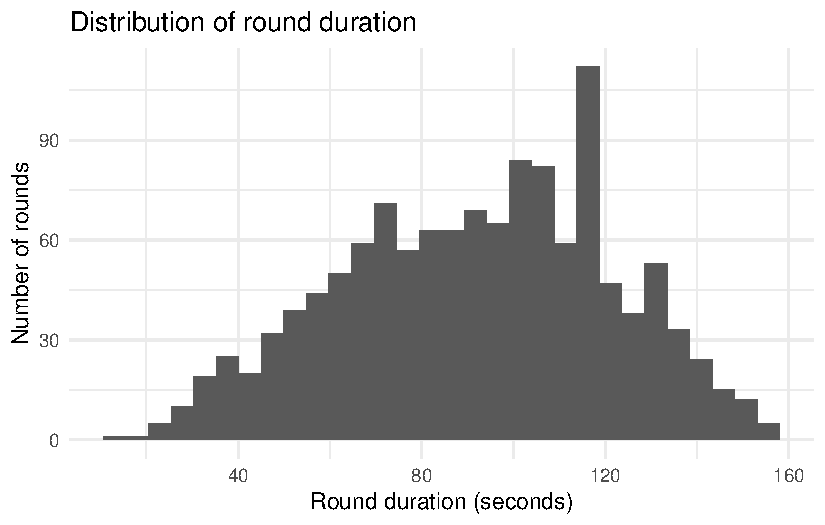
\includegraphics[keepaspectratio]{cs2_dataset_overview_files/figure-pdf/unnamed-chunk-16-1.pdf}}

\begin{Shaded}
\begin{Highlighting}[]
\FunctionTok{save\_pdf}\NormalTok{(p\_duration, }\StringTok{"03\_round\_duration\_distribution.pdf"}\NormalTok{)}
\end{Highlighting}
\end{Shaded}

\subsubsection{Bomb plant rate by map}\label{bomb-plant-rate-by-map}

\begin{Shaded}
\begin{Highlighting}[]
\NormalTok{plant\_summary }\OtherTok{\textless{}{-}}\NormalTok{ rounds }\SpecialCharTok{|\textgreater{}}
  \FunctionTok{group\_by}\NormalTok{(map) }\SpecialCharTok{|\textgreater{}}
  \FunctionTok{summarise}\NormalTok{(}
    \AttributeTok{total\_rounds =} \FunctionTok{n}\NormalTok{(),}
    \AttributeTok{planted\_rounds =} \FunctionTok{sum}\NormalTok{(bomb\_planted }\SpecialCharTok{\%in\%} \ConstantTok{TRUE}\NormalTok{, }\AttributeTok{na.rm =} \ConstantTok{TRUE}\NormalTok{),}
    \AttributeTok{plant\_rate\_pct =} \DecValTok{100} \SpecialCharTok{*} \FunctionTok{mean}\NormalTok{(bomb\_planted }\SpecialCharTok{\%in\%} \ConstantTok{TRUE}\NormalTok{, }\AttributeTok{na.rm =} \ConstantTok{TRUE}\NormalTok{),}
    \AttributeTok{.groups =} \StringTok{"drop"}
\NormalTok{  )}
\FunctionTok{show\_table}\NormalTok{(plant\_summary)}
\end{Highlighting}
\end{Shaded}

{\def\LTcaptype{none} % do not increment counter
\begin{longtable}[]{@{}lrrr@{}}
\toprule\noalign{}
map & total\_rounds & planted\_rounds & plant\_rate\_pct \\
\midrule\noalign{}
\endhead
\bottomrule\noalign{}
\endlastfoot
de\_dust2 & 628 & 349 & 55.57 \\
de\_mirage & 629 & 312 & 49.60 \\
\end{longtable}
}

\begin{Shaded}
\begin{Highlighting}[]
\NormalTok{p\_plant\_rate }\OtherTok{\textless{}{-}} \FunctionTok{ggplot}\NormalTok{(plant\_summary, }\FunctionTok{aes}\NormalTok{(}\AttributeTok{x =}\NormalTok{ map, }\AttributeTok{y =}\NormalTok{ plant\_rate\_pct)) }\SpecialCharTok{+}
  \FunctionTok{geom\_col}\NormalTok{() }\SpecialCharTok{+}
  \FunctionTok{geom\_text}\NormalTok{(}\FunctionTok{aes}\NormalTok{(}\AttributeTok{label =} \FunctionTok{sprintf}\NormalTok{(}\StringTok{"\%.1f\%\%"}\NormalTok{, plant\_rate\_pct)), }\AttributeTok{vjust =} \SpecialCharTok{{-}}\FloatTok{0.3}\NormalTok{) }\SpecialCharTok{+}
  \FunctionTok{scale\_y\_continuous}\NormalTok{(}\AttributeTok{limits =} \FunctionTok{c}\NormalTok{(}\DecValTok{0}\NormalTok{, }\DecValTok{100}\NormalTok{),}
                     \AttributeTok{expand =} \FunctionTok{expansion}\NormalTok{(}\AttributeTok{mult =} \FunctionTok{c}\NormalTok{(}\DecValTok{0}\NormalTok{, }\FloatTok{0.08}\NormalTok{))) }\SpecialCharTok{+}
  \FunctionTok{labs}\NormalTok{(}\AttributeTok{title =} \StringTok{"Bomb plant rate by map"}\NormalTok{, }\AttributeTok{x =} \StringTok{"Map"}\NormalTok{,}
       \AttributeTok{y =} \StringTok{"Rounds with a bomb plant (\%)"}\NormalTok{) }\SpecialCharTok{+}
  \FunctionTok{theme\_minimal}\NormalTok{()}

\NormalTok{p\_plant\_rate}
\end{Highlighting}
\end{Shaded}

\pandocbounded{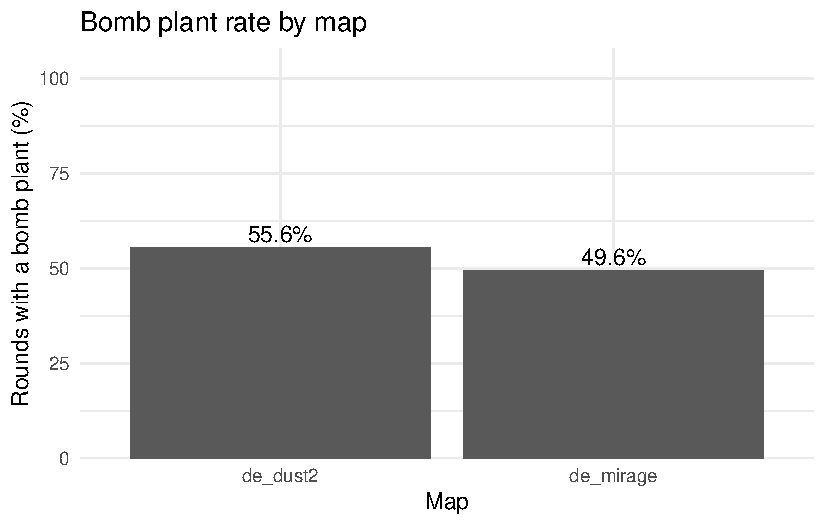
\includegraphics[keepaspectratio]{cs2_dataset_overview_files/figure-pdf/unnamed-chunk-17-1.pdf}}

\begin{Shaded}
\begin{Highlighting}[]
\FunctionTok{save\_pdf}\NormalTok{(p\_plant\_rate, }\StringTok{"03\_bomb\_plant\_rate.pdf"}\NormalTok{)}
\end{Highlighting}
\end{Shaded}

\subsubsection{Buy-type distribution by map and
side}\label{buy-type-distribution-by-map-and-side}

\begin{Shaded}
\begin{Highlighting}[]
\NormalTok{buy\_type\_summary }\OtherTok{\textless{}{-}} \FunctionTok{bind\_rows}\NormalTok{(}
\NormalTok{  rounds }\SpecialCharTok{|\textgreater{}} \FunctionTok{count}\NormalTok{(map, }\AttributeTok{buy\_type =}\NormalTok{ ct\_buy\_type, }\AttributeTok{name =} \StringTok{"rounds"}\NormalTok{) }\SpecialCharTok{|\textgreater{}}
    \FunctionTok{mutate}\NormalTok{(}\AttributeTok{side =} \StringTok{"CT"}\NormalTok{),}
\NormalTok{  rounds }\SpecialCharTok{|\textgreater{}} \FunctionTok{count}\NormalTok{(map, }\AttributeTok{buy\_type =}\NormalTok{ t\_buy\_type, }\AttributeTok{name =} \StringTok{"rounds"}\NormalTok{) }\SpecialCharTok{|\textgreater{}}
    \FunctionTok{mutate}\NormalTok{(}\AttributeTok{side =} \StringTok{"T"}\NormalTok{)}
\NormalTok{) }\SpecialCharTok{|\textgreater{}}
  \FunctionTok{group\_by}\NormalTok{(map, side) }\SpecialCharTok{|\textgreater{}}
  \FunctionTok{mutate}\NormalTok{(}\AttributeTok{percentage =} \DecValTok{100} \SpecialCharTok{*}\NormalTok{ rounds }\SpecialCharTok{/} \FunctionTok{sum}\NormalTok{(rounds)) }\SpecialCharTok{|\textgreater{}}
  \FunctionTok{ungroup}\NormalTok{()}

\FunctionTok{show\_table}\NormalTok{(buy\_type\_summary)}
\end{Highlighting}
\end{Shaded}

{\def\LTcaptype{none} % do not increment counter
\begin{longtable}[]{@{}llrlr@{}}
\toprule\noalign{}
map & buy\_type & rounds & side & percentage \\
\midrule\noalign{}
\endhead
\bottomrule\noalign{}
\endlastfoot
de\_dust2 & eco & 20 & CT & 3.18 \\
de\_dust2 & force & 105 & CT & 16.72 \\
de\_dust2 & full & 443 & CT & 70.54 \\
de\_dust2 & pistol & 60 & CT & 9.55 \\
de\_mirage & eco & 25 & CT & 3.97 \\
de\_mirage & force & 94 & CT & 14.94 \\
de\_mirage & full & 439 & CT & 69.79 \\
de\_mirage & pistol & 60 & CT & 9.54 \\
de\_mirage & NA & 11 & CT & 1.75 \\
de\_dust2 & eco & 46 & T & 7.32 \\
de\_dust2 & force & 100 & T & 15.92 \\
de\_dust2 & full & 422 & T & 67.20 \\
de\_dust2 & pistol & 60 & T & 9.55 \\
de\_mirage & eco & 44 & T & 7.00 \\
de\_mirage & force & 133 & T & 21.14 \\
de\_mirage & full & 381 & T & 60.57 \\
de\_mirage & pistol & 60 & T & 9.54 \\
de\_mirage & NA & 11 & T & 1.75 \\
\end{longtable}
}

\begin{Shaded}
\begin{Highlighting}[]
\NormalTok{p\_buy\_types }\OtherTok{\textless{}{-}} \FunctionTok{ggplot}\NormalTok{(}
\NormalTok{  buy\_type\_summary, }\FunctionTok{aes}\NormalTok{(}\AttributeTok{x =}\NormalTok{ buy\_type, }\AttributeTok{y =}\NormalTok{ percentage, }\AttributeTok{fill =}\NormalTok{ side)}
\NormalTok{) }\SpecialCharTok{+}
  \FunctionTok{geom\_col}\NormalTok{(}\AttributeTok{position =} \StringTok{"dodge"}\NormalTok{) }\SpecialCharTok{+}
  \FunctionTok{labs}\NormalTok{(}\AttributeTok{title =} \StringTok{"Buy{-}type distribution by map and side"}\NormalTok{,}
       \AttributeTok{x =} \StringTok{"Buy type"}\NormalTok{, }\AttributeTok{y =} \StringTok{"Percentage of rounds"}\NormalTok{, }\AttributeTok{fill =} \StringTok{"Side"}\NormalTok{) }\SpecialCharTok{+}
  \FunctionTok{theme\_minimal}\NormalTok{() }\SpecialCharTok{+}
  \FunctionTok{theme}\NormalTok{(}\AttributeTok{axis.text.x =} \FunctionTok{element\_text}\NormalTok{(}\AttributeTok{angle =} \DecValTok{30}\NormalTok{, }\AttributeTok{hjust =} \DecValTok{1}\NormalTok{))}

\NormalTok{p\_buy\_types}
\end{Highlighting}
\end{Shaded}

\pandocbounded{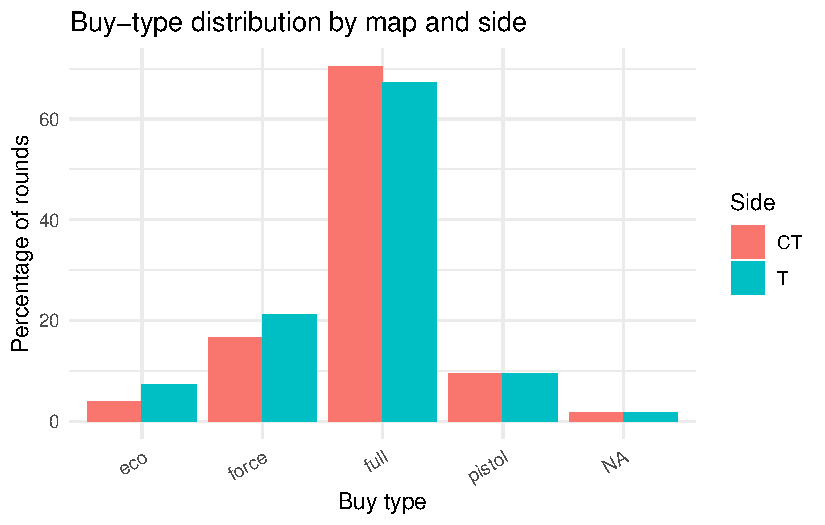
\includegraphics[keepaspectratio]{cs2_dataset_overview_files/figure-pdf/unnamed-chunk-18-1.pdf}}

\begin{Shaded}
\begin{Highlighting}[]
\FunctionTok{save\_pdf}\NormalTok{(p\_buy\_types, }\StringTok{"03\_buy\_type\_distribution.pdf"}\NormalTok{)}
\end{Highlighting}
\end{Shaded}

\subsection{4. Initial analysis ideas}\label{initial-analysis-ideas}

These comparisons are descriptive, not causal. For round-level
comparisons, use one observation per round. The state-based analyses
below select the latest snapshot at or before 30 seconds.

\subsubsection{4.1 Bomb plant and round
outcome}\label{bomb-plant-and-round-outcome}

\begin{Shaded}
\begin{Highlighting}[]
\NormalTok{plant\_outcomes }\OtherTok{\textless{}{-}}\NormalTok{ rounds }\SpecialCharTok{|\textgreater{}}
  \FunctionTok{mutate}\NormalTok{(}
    \AttributeTok{plant\_status =} \FunctionTok{case\_when}\NormalTok{(}
\NormalTok{      bomb\_planted }\SpecialCharTok{\%in\%} \ConstantTok{TRUE} \SpecialCharTok{\textasciitilde{}} \StringTok{"Planted"}\NormalTok{,}
\NormalTok{      bomb\_planted }\SpecialCharTok{\%in\%} \ConstantTok{FALSE} \SpecialCharTok{\textasciitilde{}} \StringTok{"Not planted"}\NormalTok{,}
      \ConstantTok{TRUE} \SpecialCharTok{\textasciitilde{}} \StringTok{"Unknown"}
\NormalTok{    )}
\NormalTok{  ) }\SpecialCharTok{|\textgreater{}}
  \FunctionTok{group\_by}\NormalTok{(map, plant\_status) }\SpecialCharTok{|\textgreater{}}
  \FunctionTok{summarise}\NormalTok{(}
    \AttributeTok{rounds =} \FunctionTok{n}\NormalTok{(),}
    \AttributeTok{ct\_win\_pct =} \DecValTok{100} \SpecialCharTok{*} \FunctionTok{mean}\NormalTok{(ct\_win, }\AttributeTok{na.rm =} \ConstantTok{TRUE}\NormalTok{),}
    \AttributeTok{.groups =} \StringTok{"drop"}
\NormalTok{  )}
\FunctionTok{show\_table}\NormalTok{(plant\_outcomes)}
\end{Highlighting}
\end{Shaded}

{\def\LTcaptype{none} % do not increment counter
\begin{longtable}[]{@{}llrr@{}}
\toprule\noalign{}
map & plant\_status & rounds & ct\_win\_pct \\
\midrule\noalign{}
\endhead
\bottomrule\noalign{}
\endlastfoot
de\_dust2 & Not planted & 279 & 83.51 \\
de\_dust2 & Planted & 349 & 22.64 \\
de\_mirage & Not planted & 317 & 86.12 \\
de\_mirage & Planted & 312 & 25.00 \\
\end{longtable}
}

\begin{Shaded}
\begin{Highlighting}[]
\NormalTok{plant\_site\_outcomes }\OtherTok{\textless{}{-}}\NormalTok{ rounds }\SpecialCharTok{|\textgreater{}}
  \FunctionTok{filter}\NormalTok{(bomb\_planted }\SpecialCharTok{\%in\%} \ConstantTok{TRUE}\NormalTok{, }\SpecialCharTok{!}\FunctionTok{is.na}\NormalTok{(plant\_site)) }\SpecialCharTok{|\textgreater{}}
  \FunctionTok{group\_by}\NormalTok{(map, plant\_site) }\SpecialCharTok{|\textgreater{}}
  \FunctionTok{summarise}\NormalTok{(}
    \AttributeTok{planted\_rounds =} \FunctionTok{n}\NormalTok{(),}
    \AttributeTok{ct\_win\_pct =} \DecValTok{100} \SpecialCharTok{*} \FunctionTok{mean}\NormalTok{(ct\_win, }\AttributeTok{na.rm =} \ConstantTok{TRUE}\NormalTok{),}
    \AttributeTok{.groups =} \StringTok{"drop"}
\NormalTok{  )}
\FunctionTok{show\_table}\NormalTok{(plant\_site\_outcomes)}
\end{Highlighting}
\end{Shaded}

{\def\LTcaptype{none} % do not increment counter
\begin{longtable}[]{@{}llrr@{}}
\toprule\noalign{}
map & plant\_site & planted\_rounds & ct\_win\_pct \\
\midrule\noalign{}
\endhead
\bottomrule\noalign{}
\endlastfoot
de\_dust2 & A & 199 & 26.63 \\
de\_dust2 & B & 150 & 17.33 \\
de\_mirage & A & 187 & 31.55 \\
de\_mirage & B & 125 & 15.20 \\
\end{longtable}
}

\subsubsection{4.2 Alive-player advantage at 30
seconds}\label{alive-player-advantage-at-30-seconds}

\begin{Shaded}
\begin{Highlighting}[]
\NormalTok{state\_at\_30s }\OtherTok{\textless{}{-}}\NormalTok{ round\_states\_enriched }\SpecialCharTok{|\textgreater{}}
  \FunctionTok{filter}\NormalTok{(seconds }\SpecialCharTok{\textless{}=} \DecValTok{30}\NormalTok{) }\SpecialCharTok{|\textgreater{}}
  \FunctionTok{group\_by}\NormalTok{(match\_id, round\_num) }\SpecialCharTok{|\textgreater{}}
  \FunctionTok{slice\_max}\NormalTok{(}\AttributeTok{order\_by =}\NormalTok{ seconds, }\AttributeTok{n =} \DecValTok{1}\NormalTok{, }\AttributeTok{with\_ties =} \ConstantTok{FALSE}\NormalTok{) }\SpecialCharTok{|\textgreater{}}
  \FunctionTok{ungroup}\NormalTok{() }\SpecialCharTok{|\textgreater{}}
  \FunctionTok{mutate}\NormalTok{(}
    \AttributeTok{alive\_difference =}\NormalTok{ ct\_alive }\SpecialCharTok{{-}}\NormalTok{ t\_alive,}
    \AttributeTok{alive\_advantage =} \FunctionTok{case\_when}\NormalTok{(}
\NormalTok{      alive\_difference }\SpecialCharTok{\textgreater{}} \DecValTok{0} \SpecialCharTok{\textasciitilde{}} \StringTok{"CT has more alive"}\NormalTok{,}
\NormalTok{      alive\_difference }\SpecialCharTok{\textless{}} \DecValTok{0} \SpecialCharTok{\textasciitilde{}} \StringTok{"T has more alive"}\NormalTok{,}
\NormalTok{      alive\_difference }\SpecialCharTok{==} \DecValTok{0} \SpecialCharTok{\textasciitilde{}} \StringTok{"Equal alive players"}\NormalTok{,}
      \ConstantTok{TRUE} \SpecialCharTok{\textasciitilde{}} \ConstantTok{NA\_character\_}
\NormalTok{    )}
\NormalTok{  )}

\NormalTok{alive\_outcome\_30s }\OtherTok{\textless{}{-}}\NormalTok{ state\_at\_30s }\SpecialCharTok{|\textgreater{}}
  \FunctionTok{filter}\NormalTok{(}\SpecialCharTok{!}\FunctionTok{is.na}\NormalTok{(ct\_win), }\SpecialCharTok{!}\FunctionTok{is.na}\NormalTok{(alive\_advantage)) }\SpecialCharTok{|\textgreater{}}
  \FunctionTok{group\_by}\NormalTok{(alive\_advantage) }\SpecialCharTok{|\textgreater{}}
  \FunctionTok{summarise}\NormalTok{(}
    \AttributeTok{rounds =} \FunctionTok{n}\NormalTok{(),}
    \AttributeTok{ct\_win\_pct =} \DecValTok{100} \SpecialCharTok{*} \FunctionTok{mean}\NormalTok{(ct\_win, }\AttributeTok{na.rm =} \ConstantTok{TRUE}\NormalTok{),}
    \AttributeTok{.groups =} \StringTok{"drop"}
\NormalTok{  )}
\FunctionTok{show\_table}\NormalTok{(alive\_outcome\_30s)}
\end{Highlighting}
\end{Shaded}

{\def\LTcaptype{none} % do not increment counter
\begin{longtable}[]{@{}lrr@{}}
\toprule\noalign{}
alive\_advantage & rounds & ct\_win\_pct \\
\midrule\noalign{}
\endhead
\bottomrule\noalign{}
\endlastfoot
CT has more alive & 300 & 81.00 \\
Equal alive players & 749 & 50.73 \\
T has more alive & 208 & 19.23 \\
\end{longtable}
}

\subsubsection{4.3 Equipment and economy advantage at 30
seconds}\label{equipment-and-economy-advantage-at-30-seconds}

\begin{Shaded}
\begin{Highlighting}[]
\NormalTok{economy\_summary }\OtherTok{\textless{}{-}}\NormalTok{ round\_states\_enriched }\SpecialCharTok{|\textgreater{}}
  \FunctionTok{mutate}\NormalTok{(}
    \AttributeTok{equipment\_difference =}\NormalTok{ ct\_equipment }\SpecialCharTok{{-}}\NormalTok{ t\_equipment,}
    \AttributeTok{money\_difference =}\NormalTok{ ct\_money }\SpecialCharTok{{-}}\NormalTok{ t\_money}
\NormalTok{  ) }\SpecialCharTok{|\textgreater{}}
  \FunctionTok{group\_by}\NormalTok{(match\_id, round\_num) }\SpecialCharTok{|\textgreater{}}
  \FunctionTok{filter}\NormalTok{(seconds }\SpecialCharTok{\textless{}=} \DecValTok{30}\NormalTok{) }\SpecialCharTok{|\textgreater{}}
  \FunctionTok{slice\_max}\NormalTok{(}\AttributeTok{order\_by =}\NormalTok{ seconds, }\AttributeTok{n =} \DecValTok{1}\NormalTok{, }\AttributeTok{with\_ties =} \ConstantTok{FALSE}\NormalTok{) }\SpecialCharTok{|\textgreater{}}
  \FunctionTok{ungroup}\NormalTok{() }\SpecialCharTok{|\textgreater{}}
  \FunctionTok{filter}\NormalTok{(}
    \SpecialCharTok{!}\FunctionTok{is.na}\NormalTok{(ct\_win),}
    \SpecialCharTok{!}\FunctionTok{is.na}\NormalTok{(equipment\_difference),}
    \SpecialCharTok{!}\FunctionTok{is.na}\NormalTok{(money\_difference)}
\NormalTok{  ) }\SpecialCharTok{|\textgreater{}}
  \FunctionTok{mutate}\NormalTok{(}
    \AttributeTok{equipment\_advantage =} \FunctionTok{case\_when}\NormalTok{(}
\NormalTok{      equipment\_difference }\SpecialCharTok{\textgreater{}} \DecValTok{0} \SpecialCharTok{\textasciitilde{}} \StringTok{"CT higher equipment"}\NormalTok{,}
\NormalTok{      equipment\_difference }\SpecialCharTok{\textless{}} \DecValTok{0} \SpecialCharTok{\textasciitilde{}} \StringTok{"T higher equipment"}\NormalTok{,}
\NormalTok{      equipment\_difference }\SpecialCharTok{==} \DecValTok{0} \SpecialCharTok{\textasciitilde{}} \StringTok{"Equal equipment"}
\NormalTok{    )}
\NormalTok{  ) }\SpecialCharTok{|\textgreater{}}
  \FunctionTok{group\_by}\NormalTok{(equipment\_advantage) }\SpecialCharTok{|\textgreater{}}
  \FunctionTok{summarise}\NormalTok{(}
    \AttributeTok{rounds =} \FunctionTok{n}\NormalTok{(),}
    \AttributeTok{ct\_win\_pct =} \DecValTok{100} \SpecialCharTok{*} \FunctionTok{mean}\NormalTok{(ct\_win, }\AttributeTok{na.rm =} \ConstantTok{TRUE}\NormalTok{),}
    \AttributeTok{mean\_equipment\_difference =} \FunctionTok{mean}\NormalTok{(equipment\_difference, }\AttributeTok{na.rm =} \ConstantTok{TRUE}\NormalTok{),}
    \AttributeTok{mean\_money\_difference =} \FunctionTok{mean}\NormalTok{(money\_difference, }\AttributeTok{na.rm =} \ConstantTok{TRUE}\NormalTok{),}
    \AttributeTok{.groups =} \StringTok{"drop"}
\NormalTok{  )}
\FunctionTok{show\_table}\NormalTok{(economy\_summary)}
\end{Highlighting}
\end{Shaded}

{\def\LTcaptype{none} % do not increment counter
\begin{longtable}[]{@{}lrrrr@{}}
\toprule\noalign{}
equipment\_advantage & rounds & ct\_win\_pct &
mean\_equipment\_difference & mean\_money\_difference \\
\midrule\noalign{}
\endhead
\bottomrule\noalign{}
\endlastfoot
CT higher equipment & 793 & 68.73 & 9770.11 & 5265.07 \\
Equal equipment & 6 & 50.00 & 0.00 & -616.67 \\
T higher equipment & 458 & 25.11 & -8162.12 & -5150.87 \\
\end{longtable}
}

\subsubsection{4.4 Health and armor advantage at 30
seconds}\label{health-and-armor-advantage-at-30-seconds}

\begin{Shaded}
\begin{Highlighting}[]
\NormalTok{health\_armor\_summary }\OtherTok{\textless{}{-}}\NormalTok{ round\_states\_enriched }\SpecialCharTok{|\textgreater{}}
  \FunctionTok{mutate}\NormalTok{(}
    \AttributeTok{hp\_difference =}\NormalTok{ ct\_hp }\SpecialCharTok{{-}}\NormalTok{ t\_hp,}
    \AttributeTok{armor\_difference =}\NormalTok{ ct\_armor }\SpecialCharTok{{-}}\NormalTok{ t\_armor}
\NormalTok{  ) }\SpecialCharTok{|\textgreater{}}
  \FunctionTok{group\_by}\NormalTok{(match\_id, round\_num) }\SpecialCharTok{|\textgreater{}}
  \FunctionTok{filter}\NormalTok{(seconds }\SpecialCharTok{\textless{}=} \DecValTok{30}\NormalTok{) }\SpecialCharTok{|\textgreater{}}
  \FunctionTok{slice\_max}\NormalTok{(}\AttributeTok{order\_by =}\NormalTok{ seconds, }\AttributeTok{n =} \DecValTok{1}\NormalTok{, }\AttributeTok{with\_ties =} \ConstantTok{FALSE}\NormalTok{) }\SpecialCharTok{|\textgreater{}}
  \FunctionTok{ungroup}\NormalTok{() }\SpecialCharTok{|\textgreater{}}
  \FunctionTok{filter}\NormalTok{(}\SpecialCharTok{!}\FunctionTok{is.na}\NormalTok{(ct\_win)) }\SpecialCharTok{|\textgreater{}}
  \FunctionTok{mutate}\NormalTok{(}
    \AttributeTok{hp\_advantage =} \FunctionTok{case\_when}\NormalTok{(}
\NormalTok{      hp\_difference }\SpecialCharTok{\textgreater{}} \DecValTok{0} \SpecialCharTok{\textasciitilde{}} \StringTok{"CT higher HP"}\NormalTok{,}
\NormalTok{      hp\_difference }\SpecialCharTok{\textless{}} \DecValTok{0} \SpecialCharTok{\textasciitilde{}} \StringTok{"T higher HP"}\NormalTok{,}
\NormalTok{      hp\_difference }\SpecialCharTok{==} \DecValTok{0} \SpecialCharTok{\textasciitilde{}} \StringTok{"Equal HP"}\NormalTok{,}
      \ConstantTok{TRUE} \SpecialCharTok{\textasciitilde{}} \ConstantTok{NA\_character\_}
\NormalTok{    )}
\NormalTok{  ) }\SpecialCharTok{|\textgreater{}}
  \FunctionTok{group\_by}\NormalTok{(hp\_advantage) }\SpecialCharTok{|\textgreater{}}
  \FunctionTok{summarise}\NormalTok{(}
    \AttributeTok{rounds =} \FunctionTok{n}\NormalTok{(),}
    \AttributeTok{ct\_win\_pct =} \DecValTok{100} \SpecialCharTok{*} \FunctionTok{mean}\NormalTok{(ct\_win, }\AttributeTok{na.rm =} \ConstantTok{TRUE}\NormalTok{),}
    \AttributeTok{mean\_hp\_difference =} \FunctionTok{mean}\NormalTok{(hp\_difference, }\AttributeTok{na.rm =} \ConstantTok{TRUE}\NormalTok{),}
    \AttributeTok{mean\_armor\_difference =} \FunctionTok{mean}\NormalTok{(armor\_difference, }\AttributeTok{na.rm =} \ConstantTok{TRUE}\NormalTok{),}
    \AttributeTok{.groups =} \StringTok{"drop"}
\NormalTok{  )}
\FunctionTok{show\_table}\NormalTok{(health\_armor\_summary)}
\end{Highlighting}
\end{Shaded}

{\def\LTcaptype{none} % do not increment counter
\begin{longtable}[]{@{}lrrrr@{}}
\toprule\noalign{}
hp\_advantage & rounds & ct\_win\_pct & mean\_hp\_difference &
mean\_armor\_difference \\
\midrule\noalign{}
\endhead
\bottomrule\noalign{}
\endlastfoot
CT higher HP & 551 & 68.42 & 95.50 & 120.13 \\
Equal HP & 342 & 51.75 & 0.00 & 27.62 \\
T higher HP & 364 & 29.95 & -76.66 & -84.38 \\
\end{longtable}
}

\subsection{Notes and interpretation}\label{notes-and-interpretation}

\begin{itemize}
\tightlist
\item
  \texttt{rounds.parquet} contains round-level records;
  \texttt{round\_states.parquet} contains multiple time snapshots per
  round.
\item
  \texttt{round\_states\_enriched.parquet} adds round-level information
  to each snapshot. The row count should normally remain the same as the
  original snapshot data.
\item
  Missing \texttt{seconds\_since\_plant} and \texttt{plant\_site} values
  may be expected in rounds or snapshots where the bomb has not been
  planted.
\item
  The snapshot-level alive-advantage summary in section 2.2 weights
  rounds with more snapshots more heavily. Use the
  one-snapshot-per-round analysis in section 4.2 for a more comparable
  round-level description.
\item
  The 30-second analyses use the latest available snapshot at or before
  30 seconds; it may not be exactly 30 seconds.
\item
  Figures are saved as PDF files in \texttt{../reports/figures}.
\end{itemize}




\end{document}
